\documentclass[10pt,a4paper]{report}

% Page layout
%\usepackage{a4wide}
\usepackage[top={25mm}, right={25mm}, bottom={25mm}, left={25mm}]{geometry}

% For math typesetting it's standard to use the following
\usepackage{amsmath}
\usepackage{amssymb}

\usepackage{supertabular}

% For \includegraphics
\usepackage{graphicx}

\usepackage{verbatim}

\usepackage{rotating}

% Have clickable items in table of contents, index, etc.
% (Only in pdf version)
\usepackage{url}
%\usepackage{hyperref}

%\hypersetup{
%  pdftitle={FEAST - Finite Element Analysis & Solution Tools. Technical Documentation},
%  pdfauthor={Ch. Becker, S. Buijssen, M. Grajewski, S. Kilian, S. Turek, H. Wobker},
%  pdfsubject={Technical Documentation},
%  pdfkeywords={FEAST, finite elements}
%}

\newcommand{\scarc}{\textsc{ScaRC} }
\newcommand{\devisor}{\textsc{DeViSoR} }

\bibliographystyle{abbrv}

%%%%%%%%%%%%%%%%%%%%%%%%%%%%%%%%%%%%%%%%%%%%%%%%%%%%%%%%%%
%% Weil ich zu faul war, immer das (s. ...) zu tippen   %%
%%%%%%%%%%%%%%%%%%%%%%%%%%%%%%%%%%%%%%%%%%%%%%%%%%%%%%%%%%
\newcommand{\reff}[1]{(s. Kap. \ref{#1})}


%%%%%%%%%%%%%%%%%%%%%%%%%%%%%%%%%%%%%%%%%%%%%%%%%%%%%%%%%%%
%%     Definition einer eigenen Abbildungsumgebung       %%
%%%%%%%%%%%%%%%%%%%%%%%%%%%%%%%%%%%%%%%%%%%%%%%%%%%%%%%%%%%

\newenvironment{abb}{\begin{figure}[h!]\centering }{\end{figure}}


%%%%%%%%%%%%%%%%%%%%%%%%%%%%%%%%%%%%%%%%%%%%%%%%%%%%%%%%%%%
%%         Definition einer leckeren Code-Umgebung       %%
%%%%%%%%%%%%%%%%%%%%%%%%%%%%%%%%%%%%%%%%%%%%%%%%%%%%%%%%%%%


% counter for code environment
\newcounter{codecount}
%\setcounter{codecount}{0}

% the environment itself
\newsavebox{\codecaption}
\newlength{\codewidth}
\newenvironment{code}[2]{%
  \begin{center}%
    \vrule%
    \refstepcounter{codecount}%
%\sbox{\codecaption}{\textit{Sample \arabic{codecount}: #1}}%
    \sbox{\codecaption}{Sample \arabic{codecount}: #1}%
    \label{#2}%
    \begin{small}%
      \begin{minipage}{0.9\textwidth}%
        \hrule\vspace*{5pt}%
        \setlength{\codewidth}{0.98\textwidth}
        \begin{minipage}{\codewidth}%
          \begin{center}
            \vspace*{5pt}
            \addtolength{\codewidth}{-10pt} % 2x 5pt to have equal top, left, bottom and right margin
            \begin{minipage}{\codewidth}%
            }{%
            \end{minipage}
          \end{center}
          \vspace*{5pt}%
        \end{minipage}%
        \hspace*{5pt}\hrule%
      \end{minipage}%
    \end{small}%
    \vrule%
 \\[0.5ex] \usebox{\codecaption}%
 \end{center}%
}

\parindent0cm
\parskip1em
\renewcommand{\arraystretch}{1.5}

\begin{document}

\begin{titlepage}

\vspace*{4cm}

\begin{center}

{\Huge FEAST}\\[2cm] 
{\huge Finite Element Analysis \& Solution Tools}\\[0.5cm] 

{\LARGE Technical Documentation}\\[3cm]

\vspace*{0.5cm}

{\large
 Ch.~Becker, S.~Buijssen, M.~Grajewski,\\[1em]
 S.~Kilian, S.~Turek, H.~Wobker}

\vspace*{2cm}

\today

\vspace*{2cm}

Institut f{\"u}r Angewandte Mathematik \& Simulation, Universit{\"a}t Dortmund, Germany \\[0.5em]
telephone: +49 231 755 5934\qquad fax: +49 231 755 5933 \\[0.5em]
WWW: http://www.featflow.de/feast, Email:feast@mathematik.uni-dortmund.de

\end{center}

\end{titlepage}


\tableofcontents

%######################################################################

\chapter{Introduction}


Current trends in the software development for the numerical solving of Partial Differential Equations (PDEs), 
and here in particular for Finite Element (FEM) approaches, 
go clearly towards object oriented techniques and adaptive methods in any sense. 
Hereby the employed data and solver structures, and especially the matrix structures, are often in contradiction to modern hardware platforms. As a result, the observed computational efficiency is far 
away from expected peak rates of several GFLOP/s nowadays, and the "real life" gap will even further 
increase. Since high performance calculations 
may be only reached by explicitly 
exploiting "caching in" and "pipelining" in combination with sequentially stored
arrays (using special machine optimised linear algebra libraries), the corresponding 
realisation seems to be "easier" for simple Finite Difference approaches. So, the question arises 
how to perform similar techniques for much more sophisticated Finite Element codes.

These discrepancies between modern mathematical approaches and computational 
demands for highly structured data often lead to unreasonable calculation times for "real world" problems, 
e.g.\ {\em Computational Fluid Dynamics} (CFD) calculations in 3D, as can be seen from recent benchmarks
\cite{TurekSchaeferRannacher1998} for commercial as well as research codes. Hence, strategies for efficiency enhancement
are necessary, not only from the mathematical (algorithms, discretisations) 
but also from the software point of view.
To realise some of the aformentioned necessary improvements, we develope the new Finite Element package 
({\bf FEAST} 
-- {\bf F}inite {\bf E}lement {\bf A}nalysis \& {\bf S}olution {\bf T}ools). 
This package is based on the following concepts:

\begin{itemize}
\item (recursive) "Divide and Conquer" strategies,
\item hierarchical data, solver and matrix structures,
\item {\sc ScaRC} as generalization of multigrid and domain decomposition techniques,
\item frequent use of machine optimised linear algebra routines, 
\item all typical Finite Element facilities included.
\end{itemize}
%
%
The result is a flexible software package with special emphasis on:
%
\begin{itemize}
\item (closer to) peak performance on modern processors,
\item typical multigrid behaviour w.r.t.\ efficiency and robustness,
\item parallelisation tools directly included on low level,
\item open for different adaptivity concepts ($r$- and $h$-adaptivity),
\item low storage requirements, 
\item application to many "real life" problems possible.
\end{itemize}

\noindent
Figure \ref{skizze} shows the general structure of the FEAST package:

\begin{figure}[!h]
\begin{center}
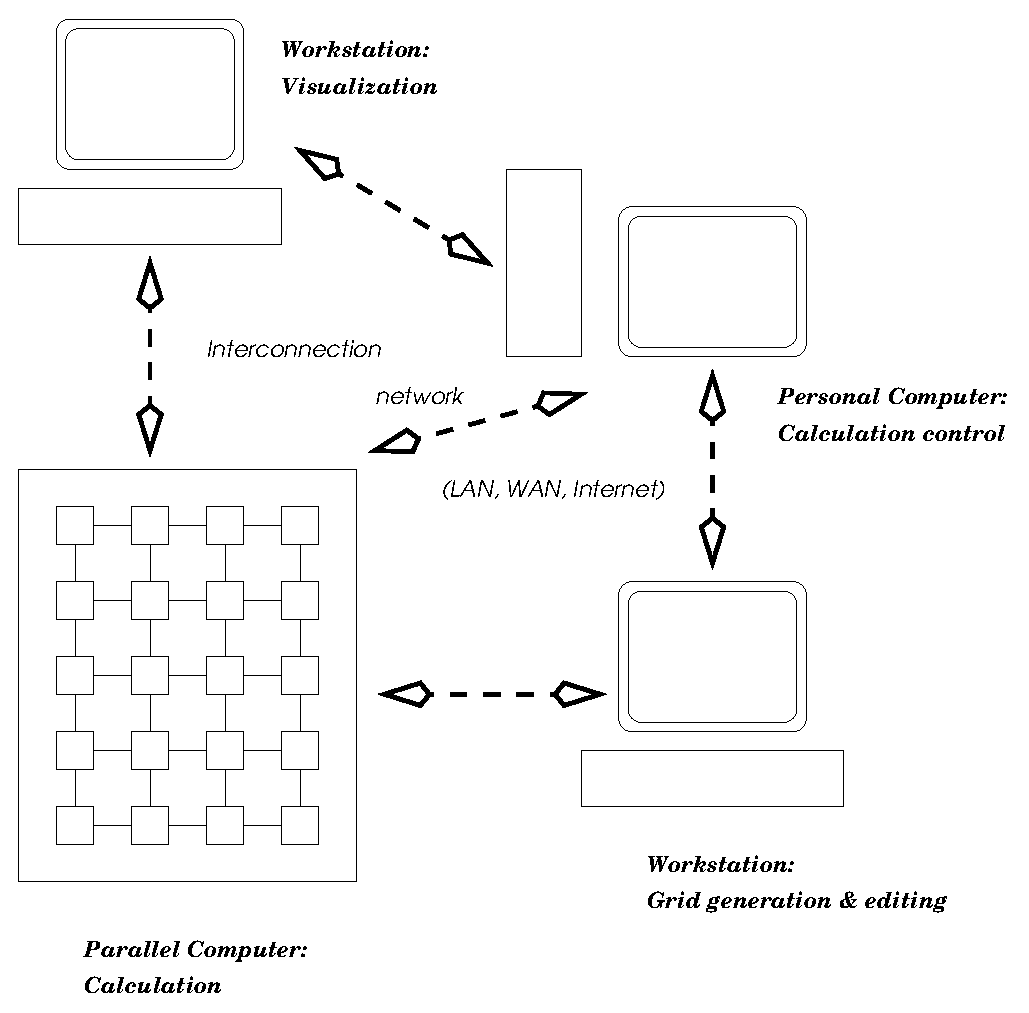
\includegraphics[scale=0.3]{../psfiles/net.eps}\hspace*{1cm}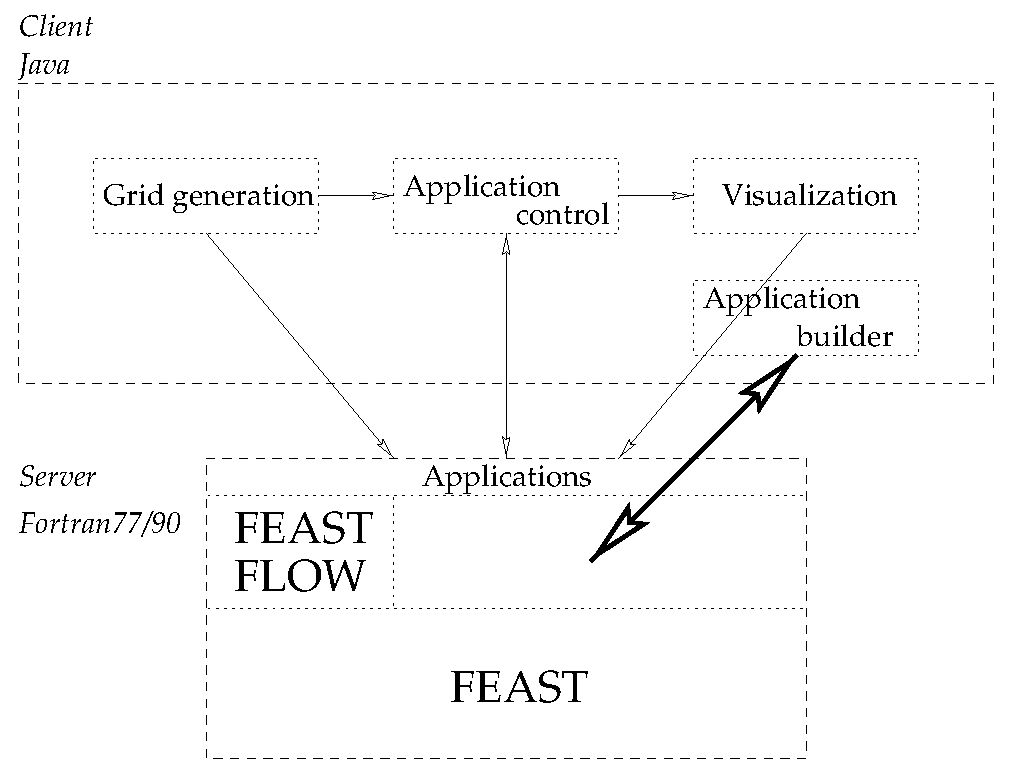
\includegraphics[scale=0.34]{../psfiles/skizze.eps}
\end{center}
\label{skizze}
\caption{FEAST structure and configuration}
\end{figure}

As programming language Fortran (77 and 90) is used. The explicit use of the
two Fortran dialects arises from following observations. For Fortran77 very
efficient and well tried compilers are available which allow to exploit much of the machine performance. 
Furthermore, it is possible
to reuse many reliable parts of the predecessor packages FEAT2D, FEAT3D
and FEATFLOW \cite{TurekBecker1999}. On the other hand Fortran77 is not more than
a better "macro assembler", the very limited language constructs
make the project work very hard. In addtition to that, F77 is no longer the current standard,
so support of this language will stop in near future. And which developer can be
motivated to program in F77?

F90 on the other hand is the new standard and provides new helpful features like records, dynamic memory 
allocation, etc. But there are several disadvantages. The language is very overloaded and the realisation
of some features like pointers is not succeeded. More severe, the compilers for Fortran 90 have not reached
the amount of stability and robustness yet like their Fortran 77 counterparts.  

The compromise is to implement the time critical routines from the numerical
linear algebra in F77, while the administrative routines are based on F90.

The pre-- and postprocessing is mainly handled by Java based program parts. 
Configuring a high performance computer as a FEAST server, the user shall be able to perform the 
remote calculation by a FEAST client. 
 

%#####################################################################



In the following we give examples for "real" computational efficiency results of typical 
numerical tools which help to motivate our hierarchical data, solver and 
matrix structures. For a better understanding, we illustrate shortly in the subsequent chapter the 
corresponding solution technique {\sc ScaRC} ({\bf Sca}lable {\bf R}ecursive {\bf C}lustering) in 
combination with the overall "Divide and Conquer" philosophy. This solver concept forms an essential part
of {\sc FEAST}. 
We discuss how typical multigrid rates can be achieved on parallel 
as well as sequential computers with a very high computational efficiency.

The typical situation in high performance computing today shows the following situation:


{\bf Example}: STAR-CD ($k-\epsilon$), 500 000 cells (by Daimer Chrysler),
SGI Origin2000 (6 CPUs), 6.5 CPU h

\begin{table}[!h]
\begin{center}
\begin{tabular}{|c||c|c||c|} \hline
{\bf Quantity}     & {\bf Experiment}  & {\bf Simulation}& {\bf Difference}\\ \hline
%
Drag (`$c_w$') & 0.165 & 0.317& {\bf 92 \%} \\
Lift (`$c_a$')   & -0.083 & -0.127& {\bf 53 \%} \\ \hline
\end{tabular}
\end{center}
\caption{Star-CD Experiment and Simulation}
\end{table}


\begin{figure}[!h]
\begin{center}
\begin{rotate}{270}
\includegraphics[scale=0.3]{../psfiles/sae.eps.0}
\end{rotate}
\hspace*{7.25cm}\begin{turn}{270}
 \includegraphics[scale=0.3]{../psfiles/sae.eps.1}
\end{turn}
\end{center}
\caption{Star-CD Simulation}
\end{figure}


%#####################################################################




\section{Main Principles in FEAST}

\subsection{Hierarchical data, solver and matrix structures}


One of the most important principles in {\sc FEAST} is to apply consequently a 
{\it (Recursive) Divide and Conquer} strategy. The solution of the complete "global" problem is recursively 
split into smaller "independent" subproblems on "patches" as part of the complete set of unknowns. 
Thus the two major aims in this splitting procedure which can be performed by hand or via self--adaptive 
strategies are:

\begin{itemize}
\item {\em Find locally structured parts.}
\item {\em Find locally anisotropic parts.}
\end{itemize}

Based on "small" structured subdomains on the lowest level (in fact, even one single or a small number of 
elements is allowed), the "higher--level" substructures are generated via clustering of "lower--level" 
parts such that algebraic or 
geometric irregularities are hidden inside the new "higher-level" patch. Additional background information
on this strategy is given in the following sections which describe the corresponding 
solvers related to each stage.

Figures \ref{FIG_f1s} and \ref{FIG_f2s} illustrate exemplarily the employed data structure for a (coarse) triangulation of a 
given domain and its recursive partitioning into several kinds of substructures.

\begin{figure}[htbp]
\begin{center}
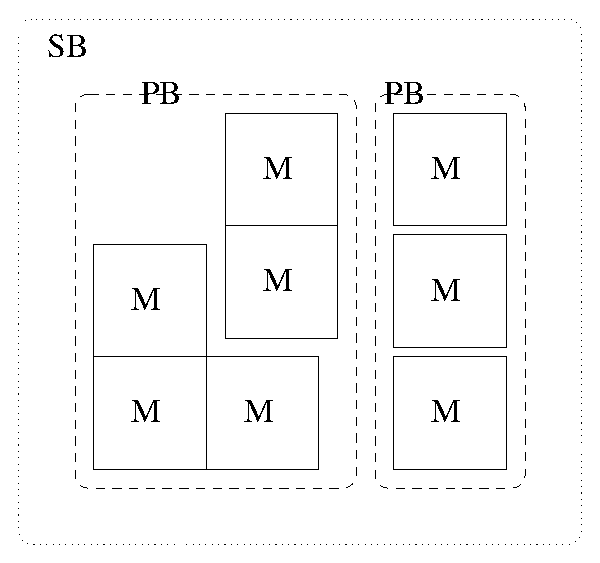
\includegraphics[scale=0.4]{../psfiles/ds1.eps} \hspace*{1cm} 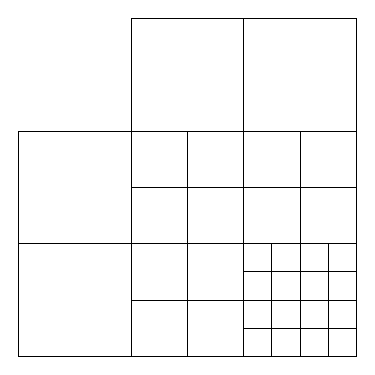
\includegraphics[scale=0.6]{../psfiles/ds2.eps}
\end{center}
\caption{FEAST domain structure}
\label{FIG_f1s}
\end{figure}

According to this decomposition, a corresponding data tree -- the skeleton of the partitioning strategy 
-- describes the hierarchical decomposition process. It consists of a specific collection of elements, 
macros, matrix blocks (MB), parallel blocks (PB), subdomain blocks (SB), etc.

\begin{figure}[htbp]
\begin{center}
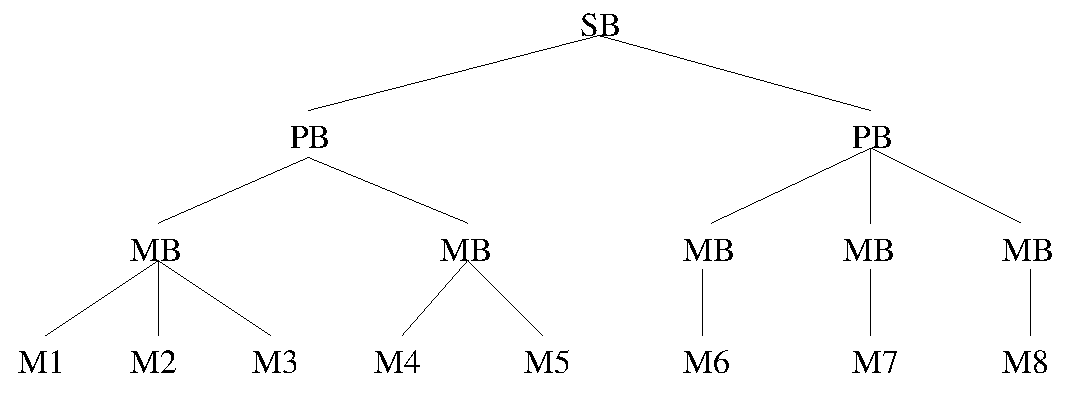
\includegraphics[scale=0.4]{../psfiles/baum.eps}
\end{center}
\caption{FEAST data tree}
\label{FIG_f2s}
\end{figure}

The {\em atomic units} in our decomposition are the "macros" which may be of type {\bf structured} 
(as $n \times n$ collection of quadrilaterals (in 2D) with local band matrices) or 
{\bf unstructured} (any collection of elements, for instance in the case of fully adaptive local grid 
refinement). These "macros" (one or several) can be clustered to build a "matrix block" which 
contains the "local matrix parts": only here is the complete matrix information stored.
Higher level constructs are "parallel blocks" (for the parallel distribution and the realisation of the load balancing) and "subdomain blocks" 
(with special conformity rules with respect to grid refinement and applied discretisation spaces). 
They all together build the complete domain, resp. the complete set of unknowns. It is important to realise 
that each stage in this hierarchical tree can act as independent "father" in relation to its 
"child" substructures. At the same time, it can act as a "child" another phase of the solution 
process (inside of the {\sc ScaRC} solver, see below).

According to this data structure and with respect to the following solver engine
Scarc in FEAST every vector belongs to one hierachical layer Subdomain (SD), Parallelblock (PB) 
and Matrixblock (MB). This concerns the way of data exchange and synchronisation.
If you e.g. perform an exchange operation to a PB-vector, then the vector is modified only
on the PB boundaries to have the same values, but not on the outer boundaries.

\subsection{Generalised solver strategy {\sc ScaRC}}

In short form our long time experience with the numerical and computational runtime behaviour of typical 
multigrid (MG) and Domain Decomposition (DD) solvers can be concluded as follows:

\subsubsection{Some observations from standard multigrid approaches:}

While in fact the numerical convergence behaviour of (optimised) multigrid is very satisfying with 
respect to robustness and efficiency requirements, there still remain some "open" problems: often 
the parallelisation of powerful recursive smoothers (like SOR or ILU) leads to performance degradations 
since they can be realised only in a blockwise sense. Thus it is often not clear how the nice 
numerical behaviour in sequential codes for complicated geometric structures or local anisotropies can be 
reached in parallel computations. And additionally, the communication overhead especially on 
coarser grid levels dominates the total CPU time.
Even more important is the "computational observation" that the 
realised performance on modern platforms is often far beyond (sometimes less than 1 \%) the expected 
peak performance. Many codes often reach much less than 50 MFLOP/s, and this on computers which are said 
(by the vendors) to run with several GFLOP/s peak performance. The reason is simply that 
the single components in multigrid (smoother, defect calculation, grid transfer) perform too few 
arithmetic work with respect to each data exchange such that the facilities of modern superscalar 
architectures are poorly exploitable. In contrast,  we will show that in fact 30 -- 70 \% 
are within reach with appropriate techniques.

\subsubsection{Some observations from standard Domain Decomposition approaches:}


In contrast to standard multigrid, the parallel efficiency is much higher, at least as long as 
no large overlap region between processors must be exchanged. While {\em overlapping} DD methods do not require additional coarse grid problems (however the implementation in 3D for complicated domains or 
for complex Finite Element spaces is a hard job), {\em non-overlapping} DD approaches require 
certain coarse grid problems, as the BPS preconditioner for instance which may lead again to several 
numerical and 
computational problems, depending on the geometrical structure or the used discretisation spaces. 
However the most important difference between Domain Decomposition and multigrid are the (often) 
much worse convergence rates of DD although at the same time more arithmetic work is done on 
each processor.


As a conclusion improvements are enforced by the facts that the {\bf convergence behaviour} is often quite sensitive with respect to (local) geometric/ algebraic {\bf anisotropies} (in "real life" 
configurations), and that the performed {\bf arithmetic work} (which allows the high performance) is often 
restricted by (un)necessary {\bf data exchanges}.


An additional observation which is strongly related to the previous data structure in combination 
with the specific hierarchical {\sc ScaRC} solver is illustrated in the following figure. We show the 
resulting "optimal" mesh from a numerical simulation of R.Becker/R.Rannacher for "Flow around the cylinder" 
which was adaptively refined via rigorous a--posteriori error control mechanisms specified for the required 
drag coefficient (\cite{RannacherBecker1996}).

\begin{figure}[htbp]
\begin{center}
\hspace*{-0.35cm}
 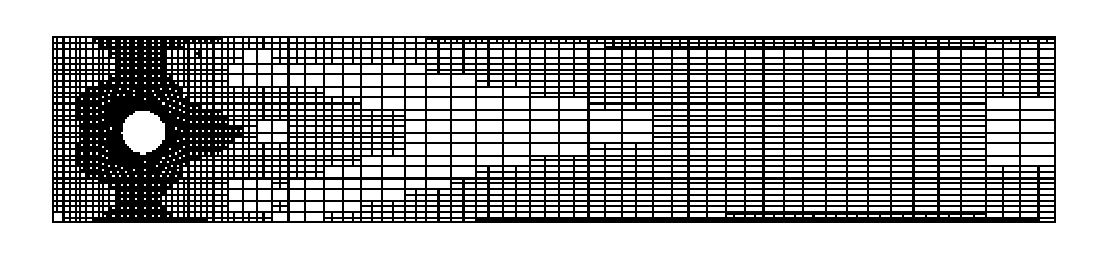
\includegraphics[scale=0.70]{../psfiles/optgrid.eps}
\end{center}
\vspace*{-0.5cm}
\caption{"Optimal grid" via a--posteriori error estimation}
\end{figure}

As can be seen the adaptive grid refinement techniques are needed only locally, near the boundaries, while 
mostly regular substructures (up to 90 \%) can be used in the interior of the domain. 
This is a quite typical result and shows that even for (more or less) complex flow simulations 
(here as a prototypical example) locally blockwise structured meshes can be applied: 
these regions can be detected and exploited by the given hierarchical strategies.

The {\sc ScaRC} approach consists of a separated multigrid approach for every hierarchical
layer, whereby the multigrid scheme on the outest layer (subdomain layer)
gives the final result. The smoothing step of the multigrid method is
based on the following notation:

\vspace*{0.2cm}

{ {Smoothing on level $h$ for $A_h x=b_h$:}}


\begin{itemize}
\item {\bf global} outer block Jacobi scheme (with averaging operator `M')
\[ x^{l+1} = x^l - \omega_g \tilde{A}^{-1}_{h,M} (A_h x^l - b_h) \]
with $\tilde{A}^{-1}_{h,M} := M \circ \tilde{A}^{-1}_{h}$ \,,\,
$\displaystyle \tilde{A}^{-1}_{h} := \sum_{i=1}^N \tilde{A}^{-1}_{h,i}$ \,,\,
$\tilde{A}_{h,i} := "A_{h|\Omega_i}"$

\item "solve" {\bf local} problems $\tilde{A}_{h,i} y_i = def_i^l := (A_h x^l - b_h)_{|\Omega_i}$ via
\[ y_i^{k+1} = y_i^k - \omega_l C^{-1}_{h,i} (\tilde{A}_{h,i} y_i^k - def_i^l) \]
with $C^{-1}_{h,i}$ preconditioner for $\tilde{A}_{h,i}$, or employ a direct solver
\end{itemize}

The local smoothing operators can be a further multigrid scheme
or any other scheme like Jacobi, Gau{\ss}--Seidel, ADI or ILU. The choice of the method depends on the local 
structure and the numerical difficulties caused by the given domain. In a first step this decision is taken by
the user to choose explicitly the method but in future it is possible to use
an "expert system" which makes this decision widely automatically. 

\vspace*{0.2cm}

There are several reasons why we explicitely use {\bf this} {\em basic iteration}:

\begin{enumerate}
\item This general form allows the splitting into matrix--vector 
multiplication, preconditioning and linear combination. All 3 components can be 
separately performed with high performance tools if available.
\item The explicit use of the complete defect $A_h x^l - b_h$ is  advantageous for certain 
techniques for implementing boundary conditions (see \cite{Turek1999h}).
\item All components in standard multigrid, i.e., smoothing, defect calculation, step--length control, 
grid transfer, are included in this {\em basic iteration}.
\end{enumerate}

Figure \ref{scarcscheme} shows an example illustration of a \scarc scheme.

%########################################################
\vspace*{0.5cm}

\begin{figure}[!h]
\hspace*{2cm}\begin{minipage}{7cm}
Standard multigrid with\\
(recursively defined)\\
block smoothers\\

\vspace*{0.2cm}
plus
\vspace*{0.2cm}

Standard Domain Decomposition\\
with minimal overlap,\\
sequence of coarse grid \\
problems via multigrid\\

\vspace*{0.2cm}
plus
\vspace*{0.2cm}

Embedded into \\
standard CG--method\\

\vspace*{-7cm}\hspace*{6cm}\includegraphics[scale=0.45]{../psfiles/groid.ps}
\end{minipage}
\caption{\scarc scheme: example}
\label{scarcscheme}
\end{figure}


%########################################################


The notation \scarc stands for:
\begin{itemize}
\item {\bf Scalable}, w.r.t. the number of global ('$l$') and local solution steps ('$k$'),
\item {\bf Recursive}, since it may be applied to more than 2 global/local levels,
\item {\bf Clustering}, since fixed or \underline{adaptive} blocking of substructures is possible.
\end{itemize}

%########################################################

\begin{figure}[!h]
\begin{center}
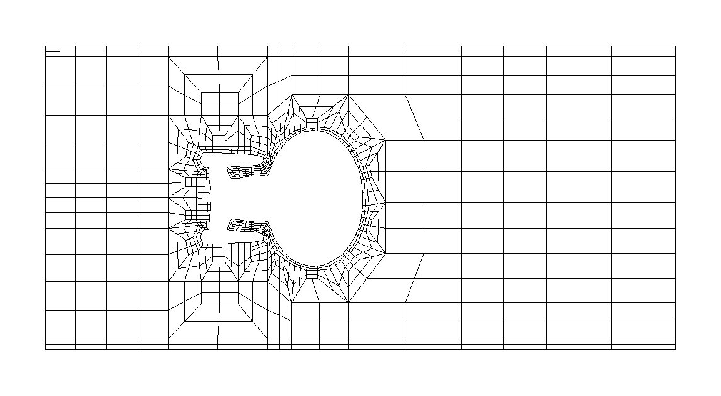
\includegraphics[width=7cm]{../psfiles/gitter1.ps}
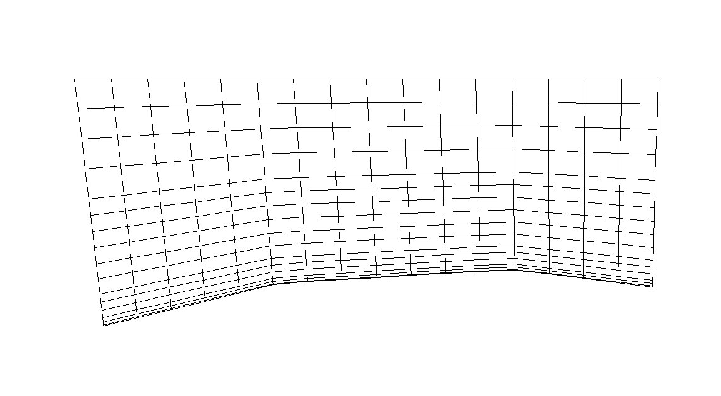
\includegraphics[width=8cm]{../psfiles/makro.ps} 
\end{center}
\caption{Example of ScaRC: 2D decomposition and zoomed (macro) element (LEVEL 3) with locally anisotropic 
refinement towards the wall}
\label{scarcexamplegrid}
\end{figure}

%########################################################

Results for a ScaRC-CG solver (smoothing steps: 1 global ScaRC; 1 local `MG-TriGS') 
for locally (an)isotropic refinement are shown in table \ref{scarcresults}.


\begin{table}[!h]
\begin{center}
\begin{tabular}{|r||c|c|c|c|}
\hline
$\#NEQ$ \phantom{  }        & \multicolumn{2}{c|}{Dirichlet 'Velocity'} & \multicolumn{2}{c|}{Neumann 'Pressure'} \\
\cline{2-5}
& $AR \approx 10$ &  $AR \approx 10^{6}$ & $AR \approx 10$ &  $AR \approx 10^{6}$ \\
\hline \hline
   $210,944$    & 0.17 ({\bf 8}) & 0.18 ({\bf 8}) & 0.21 ({\bf 9}) & 0.15 ({\bf 8}) \\
   $843,776$    & 0.17 ({\bf 8}) & 0.17 ({\bf 8}) & 0.20 ({\bf 9})  & 0.17 ({\bf 8}) \\
   $3,375,104$  & 0.18 ({\bf 9}) & 0.19 ({\bf 9}) & 0.22 ({\bf 10}) & 0.22 ({\bf 10}) \\ 
   $13,500,416$ & 0.19 ({\bf 9}) & 0.18 ({\bf 9}) & 0.23 ({\bf 10}) & 0.23 ({\bf 10}) \\ 
   \hline
\end{tabular}
\end{center}
\caption{Global (parallel) convergence rates for \scarc on configuration shown in \ref{scarcexamplegrid}}
\label{scarcresults}
\end{table}


For
more information about {\sc ScaRC} see \cite{KilianTurek1998} and \cite{Kilian2001}.


\subsection{High Performance Linear Algebra}


One of the main ideas behind the described {\it (Recursive) Divide and Conquer} approach in 
combination with the {\sc ScaRC} solver technology is to detect "locally structured parts". 
In these "local subdomains" we apply consequently "highly structured tools" as known from Finite Difference  
approaches: line-- or rowwise numbering of unknowns and storing of matrices as 
sparse bands (however the matrix entries are calculated via the Finite Element modules). 
As a result we have "optimal" data structures on each of these patches (which often correspond to 
the former introduced "matrix blocks") and we can perform very powerful 
linear algebra tools which explicitly exploit the high performance of specific 
machine optimised libraries.

We have performed several tests for different tasks 
and techniques in numerical linear algebra  on some selected hardware platforms.
In all cases we attempted to use "optimal" compiler options and 
machine optimised linear algebra libraries.

{\bf Matrix--vector multiplication:}

We examine more carefully the following variants which all are typical in the context of 
iterative schemes with sparse matrices. The test matrix is a 
typical 9--point stencil (emerging from a FE discretisation of the Poisson operator with bilinear Finite 
Elements). We perform tests for two different vector lengths $N$ and give the measured MFLOP rates which are all calculated via $20 \times N/time$ (for MV), resp., 
$2 \times N/time$ (for DAXPY). 

{\bf Sparse MV: SMV}\\
The {\em sparse MV} technique (see \ref{sparsematvecmul}) is the standard technique in Finite Element codes (and others), also well known 
as "compact storage" technique or similar: the matrix plus index arrays or lists are stored as long arrays 
containing the nonzero elements only. While this approach can be applied for arbitrary meshes and 
numberings of the unknowns, no explicit advantage of the linewise numbering can be 
exploited. We expect a massive loss of performance with respect to the possible peak rates since --- at least 
for larger problems --- no "caching in" and "pipelining" can be exploited such that the higher cost of 
memory access will dominate the resulting MFLOP rates. Results are shown in table \ref{sparsematvecmulresult}.


%#################################################################

\begin{code}{ Standard sparse matrix vector algorithm(DAXPY indexed)}{sparsematvecmul}
\begin{verbatim}
                             DO 10 IROW=1,N
                             DO 10 ICOL=KLD(IROW),KLD(IROW+1)-1
                     10      Y(IROW)=DA(ICOL)*X(KCOL(ICOL))+Y(IROW)
\end{verbatim}
\end{code}

\begin{table}[!h]
\begin{center}
\begin{tabular}{|c|c||c|c||c|} \hline
Computer     & \#Unknowns  & {\bf CM}&{\bf TL}&{\bf STO}\\ \hline
%
                                           &     8,320 & 147 & 136 & {\bf 116} \\
                                           &    33,280 & 125 & 105 & {\bf 100} \\
{\bf Alpha ES40}                           &   133,120 & 81  & 71 & {\bf 58} \\
(667 Mhz)                                  &   532,480 & 60  & 51 & {\bf  21} \\
                                           & 2,129,920 & 58  & 47 & {\bf  13} \\
                                           & 8,519,680 & 58  & 45 & {\bf  10} \\ \hline
\end{tabular}
\end{center}
\caption{Performance rates of the FEATFLOW code with
different numbering schemes (Cuthill--McKee, TwoLevel, Stochastic)
for matrix vector multiplication}
\label{sparsematvecmulresult}
\end{table}

%#################################################################

{\bf Banded MV: BMV}\\
A "natural" way to improve the {\em sparse MV} is to exploit that the matrix consists of 9 bands only. 
Hence the matrix--vector multiplication is rewritten such that now 
"band after band" are applied.  The obvious advantage of this {\em banded MV} approach is that these tasks can be performed on the basis of BLAS1--like routines which may exploit the vectorisation facilities 
of many processors (particularly on vector computers). However for "long" vector lengths the 
improvements can be absolutely disappointing: For the recent workstation/PC chip technology the processor cache dominates the resulting efficiency!


{\bf Banded blocked MV: BBMVA, BBMVL, BBMVC}\\
The final step towards highly efficient components is to rearrange the matrix--vector multiplication 
in a "blockwise" sense: for a certain set of unknowns, a corresponding part of the matrix is treated 
such that cache--optimised and fully vectorised operations can be performed. This procedure is called 
"BLAS 2+"--style since in fact certain techniques for dense matrices which are based on ideas 
from the BLAS2, resp., BLAS3 library, have now been developed for such sparse banded matrices. 
The exact procedure has to be carefully developed in dependence of the underlying FEM discretisation, 
and a more detailed description can be found in \cite{Becker2003}. 

While BBMVA has to be applied in the case of arbitrary matrix coefficients, BBMVL and BBMVC are 
modified versions which can be used under certain circumstances only (see \cite{Becker2003} for 
technical details). For example PDE's with constant coefficients as the Poisson operator but 
on a mesh which is adapted in one special direction only, allow the use of BBMVL: This is often the case for the 
Pressure--Poisson problem in flow simulations on boundary adapted meshes. 
Additionally version BBMVC may be applied for PDE's with constant coefficients on meshes with equidistant 
mesh distribution in each (local) direction separately: This is typical for tensor product meshes 
in the interior domain where the solution is mostly smooth.

Performance results for banded techniques in comparation to standard techniques are shown in table \ref{sbblasresults1}.

As example the Poisson problem with multigrid with TriGS smoother on NCC-1701D grid is calculated, corresponding
performance results are shown in table \ref{sbblasresults}.

%#################################################################


\begin{table}[!h]
\begin{center}
\begin{tabular}{|c|c|c|c|c|c|c|} \hline
2D case     & N  &{DAXPY(I)}&  \multicolumn{2}{c|}{MV} & \multicolumn{2}{c|}{MG-TriGS} \\ \hline
   &  & & V & C &  V & C \\ \hline
%
{Sun V40z     }    & $65^2$     & 1521 (422)    & 1111     &  1605    & 943      & 1178      \\
{(1800 MHz)     } & $257^2$     &  264 (106)     & 380     &  1214    & 446      & 769      \\
{`{\bf Opteron}'  } &{\bf $1025^2$}&{\bf  197 (54)}&{\bf 362}&{\bf 1140}&{\bf 333} &{\bf 570} \\ \hline

{DEC 21264     } & $65^2$     & 205 (178)    & 538     &  795    & 370      & 452      \\
{(667 MHz)     } & $257^2$     &  224 (110)     & 358     &  1010    & 314      & 487      \\
{`{\bf ES40}'  } &{\bf $1025^2$}&{\bf  78 (11)}&{\bf 158}&{\bf 813}&{\bf 185} &{\bf 401} \\ \hline


{NEC SX-6}   & $65^2$     & 1170 (422)    &1204     &  1354    & 268      & 341      \\
{(500 MHz)} & $257^2$   & 1100 (412)    &1568     &  2509    & 316      & 459      \\
{ `{\bf Vector}'   } &{\bf $1025^2$}&{\bf  1120 (420)}&{\bf 1597}&{\bf 3421}&{\bf 339} &{\bf 554} \\ \hline


{IBM POWER4}           & $65^2$   &1521 (845)    &  2064     &  3612    &  1386     &  1813     \\
{(1700 MHz)     }      & $257^2$   &1100 (227)   &  1140     &  3422    &  1048     &  1645     \\
{`{\bf Power}'}        &{\bf $1025^2$} &{\bf  390 (56)}&{\bf  550}&{\bf 2177}&{\bf  622}&{\bf  1138}\\ \hline
%
\end{tabular}
\end{center}
\caption{Performance rates for the operations DAXPY, DAXPY-I, MV and MG-TriGS for different arhitectures}
\label{sbblasresults1}
\end{table}

%#################################################################

\begin{table}[!h]
\begin{center}
\begin{tabular}{|c|c|c|c|c|} \hline
N         &    1p        &    2p       &     3p      &      4p\\ \hline
843,776    &  11.04(191)  &  5.72(368)  &  3.85(547)  &  3.45 (611) \\ 
3,381,507   &  30.36(271)  &  15.62(526) &  10.73(766) &  8.42 (976) \\
13,513,219  &  98.64(328)  &  51.04(634) &  34.79(931) &  27.80(1165) \\
54,027,267  &  367.85(301) & 198.35(559) &  129.07(859) & 107.70(1029) \\ \hline
\end{tabular}
\end{center}
\caption{CPU times and numerical MFlop rates for different numbers of CPUs
(Sun V40z, four Opteron 844 CPUs with 1800Mhz, 16 GByte memory)}
\label{sbblasresults}
\end{table}


More information in available in \cite{AltieriBeckerTurek1998}, \cite{BeckerKilianTurek1999a} and
\cite{TurekBeckerKilian2003a}.

%#################################################################
As a summary, we can draw the following conclusions:
\begin{itemize}
\item Sparse techniques are the basis for most of the recent
software packages.
\item Different numberings can lead to identical
numerical results and work (w.r.t. arith.ops and data accesses) but
to huge differences in CPU time.
\item Sparse techniques are 'slow'. The computational speed depends on the problem 
size and the kind of data access.
\end{itemize}


\subsection{Several adaptivity concepts}

As typical of modern FEM packages, we directly incorporate certain tools for grid 
generation which allow easy handling of local and global refinement or coarsening strategies:
{\bf adaptive mesh moving}, {\bf macro adaptivity} and {\bf fully local adaptivity}.

Adaptive strategies for moving mesh points, along boundaries or inner structures, allow the same 
logic structure in each "macro block", and hence the shown performance rates can be preserved. 
Additionally, we work with adaptivity concepts related to 
each "macro block". Allowing "blind" or "slave macro nodes" preserves the 
high performance facilities in each "matrix block", and is a good compromise between fully local 
adaptivity and optimal efficiency through structured data. Only in that case, that these concepts do not 
lead to satisfying results, certain macros will loose their "highly structured" features through 
the (local) use of fully adaptive techniques. On these (hopefully) few patches, the standard "sparse" 
techniques for unstructured meshes have to be applied.

\subsection{Direct integration of parallelism}

Most software packages are designed for sequential algorithms to solve a given PDE problem, and the 
subsequent parallelisation of certain methods takes often unproportionately long. 
In fact it is easy to say, but hard to realise with most software packages.  However the more important step, which makes parallelisation 
much more easier, is the design of the {\sc ScaRC} solver according to the hierarchical decomposition 
in different stages. Indeed from an algorithmic point of view, our sequential and parallel 
versions differ only as analogously Jacobi-- and Gau{\ss}--Seidel--like schemes work differently. 
Hence all parallel executions can be identically simulated on single processors which however can 
additionally improve their numerical behaviour with respect to efficiency and robustness through 
Gau{\ss}--Seidel--like mechanisms. 

Hence we only provide in {\sc FEAST} the "software" tools for including parallelism on low 
level, while the "numerical parallelism" is incorporated via our {\sc ScaRC} solver and the 
hierarchical "tree structure". However what will be "non--standard" is our concept of (adaptive) 
parallel loadbalancing 
which is oriented in "total numerical efficiency" (that means, "how much processor work is spent to achieve 
a certain accuracy, depending on the local configuration") in contrast to the "classical" criterion of 
equilibrating the number of local unknowns (see \cite{Becker2003} for detailed information and examples in {\sc FEAST}).

\section{Pre-- and Postprocessing}

\subsection{General remarks}
%
As remarked in the introduction the pre-- and postprocessing should
be realised in main tasks by a general framework of Java based programs 
called DeViSoR. DeViSoR means "Design \& Visualisation Software Resource".
This framework is intented to perform the main tasks grid generation and
editing, control of the calculation and visualisation of the results. 
These main tasks use the same ground classes (called DFC - DeViSoR Foundation
Classes) and the same user interface, so the access to the underlying 
numerical core parts are  performed in the same manner.

As intented in the introduction the various subtasks can be performed on
several machines which communicates over a network system. This allows
the user to choose the suitable system for the corresponding task, e.g.
a Silicon Graphics workstation for the visualisation. The access to
a parallel computing system should also be performed by a Java program.
This allows not only the developer of a numerical code to use a
parallel computer.

DeViSoR is planned to be an "open system" for the developing of pre-- and
postprocessing tools for FEM packages. The DeViSoR foundation classes
contain the basic tools to handle and administrate FEM typical structures.
Further applications could realise e.g. further visualisation procedures
and adaptions to several parallel computer systems.

For this project Java as implementation environment is been choosen. Though Java
is a relative "young" programming language the advantages of this system
are significant. The "write once, run anywhere" capability reduces the
implementation effort widely against combinations like C/C++/OpenGL. It
exist only one program which runs without any modification on several
different configurations like Unix workstations, Linux PCs, Windows PCs,
Macintoshs and many more. A further advantage is the core
class library for various subareas like file hand\-ling, network functions,
visualisation and user interface facilities. These classes are easy to use and
produce an pleasing output. The use of additional tools like applications
builders is not necessary. The most disadvantage of nowadays Java
implementations is the relative low performance because of the fact that
Java is an interpreted language.  However further developments like
more sophisticated interpreter with Just--In--Time compiling facilities and
especially the native Java processor will hopefully close this 
performance leak.

More information you can find in \cite{PGDeViSoR2003}.

\subsection{Preprocessing: DeViSoRGrid}

This subprogram should support the generation and editing of 2D domains.
The two main parts are the description of the domain boundary and the 
generation of the grid structure. The program supports several boundary
elements like lines, arcs and splines, further it is planned to add a
segment which consists of an Fortran subroutine which describes a
parametrisation. This allows to use an analytic description. 
Several triangular and quadrilateral elements
are supported. Extensive editing possibilities allow the user to delete, move
and adjust the boundaries and elements. For the future it is planned to implement simply automatic grid generators
for producing coarse grids. As further tasks this program should be able to read many formats from
other tools like CAD systems and professional grid generators and prepare
this data for the use in the calculation process.

\subsection{Processing: DeViSoRControl}

DeViSoRControl enables the user to control the calculation und to follow the
calculation progress. Main tasks of this program part are the distribution
of the macros to the processing nodes (at the moment manually, in future
automa\-tically), the collecting and displaying of the log information of the
processing nodes and finally the configuration of the {\sc ScaRC} algorithm with
respect to the selection of smoothing/preconditioning methods on a given
hierarchical layer, the size of smoothing steps and the stopping criterion.
Furthermore this part builds the interface to the other DeViSoR parts for
the pre-- and postprocessing. From the control part the grid program is
invoked, a grid is editing. For this grid the user selects the desired
solution method and visualise finally the results with the DeViSoRVision
program.


\subsection{Postprocessing: DeViSoRVision}

The last part in the current project is the DeViSoRVision program which
performs the visualisation task. The program offers several techniques to
visualise the results of the calculation like shading techniques, isolines,
particle tracing (planned). Furthermore it contains an animation module to
create animations for nonstationary problems. The result of the animation
can be stored in several formats like MPEG and AnimatedGIF. 




%######################################################################

\chapter{Installation}


Please perform the following prelimarary installation steps:

get \verb+feast_xx.xx.xx.tar.gz+ from \verb+www.featflow.de+

Untar the file with the command

\begin{verbatim}
gzip -d feast_xx.xx.xx.tar.gz
tar xvf feast_xx.xx.xx.tar
\end{verbatim}

This creates the following directory structure

\begin{tabbing}
feast \phantom{xxxxxxxx} \= feast \phantom{xxxxxxxxxxxxxxx} \=  -FEAST program- \\
      \> doc.pdf  \> -This document-\\
      \> README  \> -latest information-\\
      \> CHANGES \> -changes from previous versions-\\
      \> OPENBUGS \> -known and open bugs-\\
\end{tabbing}

The feast folder itself consists of the following subfolders

\begin{tabbing}
\verb+applications+ \phantom{xxxxxxxx} \= application programs \\
\verb+arch+ \> architecture dependent stuff\\
\verb+bin+ \> shell scripts and binaries\\
\verb+docs+ \> Documentation\\
\verb+fbenchmark2+  \> benchmark program \\
\verb+grids+ \> domain descriptions \\
\verb+kernel+ \> FEAST kernel sources\\
\verb+libraries+ \> external libraries \\
\verb+object+ \> folder for object files \\
\verb+outofdata+ \> stuff out of date\\
\verb+sbblas+ \> SBBLAS folder \\
\verb+sbblasbench+ \> SBBLAS benchmark folder \\
\verb+scarc+   \> folder containing the scarc algorithm descriptions\\
\verb+solver+   \> folder containing the solver algorithm descriptions
\end{tabbing}

      
Get LAM-MPI, a message passing library, from

\verb+http://www.lam-mpi.org/download+

and install it in accordance with the instructions found
in the \verb+LAM+ folder (for lsiii users: already installed) \cite{BurnsDaoudVaigl1994,SquyresLumsdaine2003}

Make sure that the environment variables \verb+MPI_INC+ and 
\verb+MPI_LIB+ point to the directories for include files and the LAM/MPI libraries, e.g.

\begin{verbatim}
setenv MPI_INC /usr/local/lam/include
setenv MPI_LIB /usr/local/lam/lib
\end{verbatim}

Make sure, that the path \verb+/usr/local/lam/bin+ is in your 
\verb+PATH+ variable.


FEAST has a global configure script located in the \verb+bin+ folder. Every
application subfolder contains a local configure script which calls the
global script with application specific options. 

\verb+configure+ tries to detect the system architecture. The architecture is
coded as following:

\verb+arch-cpu-os-mpi-compiler-blas+

The sub specifications means as follows:
\begin{itemize}
\item \verb+arch+: architecture, currently \verb+alpha,ibm,pc,sun4u,sx6+
\item \verb+cpu+: processor type, currently \verb+athlon,athlon64,athlonxp,ev6,opteron,pentium3,pentium4,+\\
\verb+pentium4m,powerpc_power4,sparcv8,sparcv9+
\item \verb+os+: operating system, currently \verb+aix,linux32,linux64,osf1,sunos,superux+
\item \verb+mpi+: MPI environment, currently \verb+dmpi,lammpi,mpich,optmpich,tsmpi+
\item \verb+compiler+: compiler, currently \verb+cf90,ifort,g95,gfortran,pgi,sunf90,xlf+
\item \verb+blas+: used BLAS library, currently \verb+atlas,blas,dxml,essl,goto,perf+
\end{itemize}


Currently, the following IDs are supported:
\verbatiminput{valid_ids}

The configure script supports the following options:
\verbatiminput{configure_help}

After configure is successfully run a makefile is created. Type \verb+make+
to compile the package and the application.


\chapter{Tutorial}

\section{A first step to FEAST Finite Element \& Solution Tools}

In the first step we want to create our grid. For this task we use
the \devisor program, which you have to load and install separately
from \url{http://www.featflow.de}.

Start \devisor with the command

\begin{verbatim}
grid3
\end{verbatim}

First we build a new domain. Go to

\verb+Domain->New Domain+ 

type \verb+1,0+ for every size in the dialog.


then we want to build the boundary description. Press the
space bar and select 

\verb+Mouse mode->Create SegmentList+, 

then
go to position (0,0) and klick the
left button, go to (1,0),(1,1),(0,1) and
klick again. To finish the boundary description press the
space bar and select 

\verb+Done!+. 

Then go to 

\verb+Domain->Save Domain As->FEAST V3+

and save the 
file under
the name \verb+~/feast/feast/grids/firstgrid.feast+.

In the next step we will create the nodes. First, we define the nodes
on the boundary. This will be done automatically by the the function

\verb+Coarse Mesh->Add multiple parameter nodes(2D)+. 

Select this function and a dialog will appear, where you can input some parameters. Change the value
of the \verb+Number of Nodes+ from 4 to 8 and click OK. This will create boundary nodes
on the edge and midpoints. One interior point has to be defined, to do this, press
space bar and select 

\verb+Mouse mode->Create Points+

and klick with the left button to
the position (0.5,0.5).

In the next step you have to define the edges. Press space bar and select 

\verb+Select+.


Klick with the left button and draw
the rubberband with pressed button so, that the nodes 1 and 2 are gathered. Then
press the E key. A new edge is created. Repeat this for the node groups
(2,9), (9,8), (8,1), (9,6), (6,7), (7,8), (5,6), (4,2), (9,4), (3,4) and (2,3)).
Then gather the complete domain, press space bar and select 

\verb+Add Quads+.

Now the grid is ready and you can finally save it.

Now we can try to start a calculation run. Go to the folder 

\verb+~/feast/feast/applications/poisson+ 

and type: \verb+./configure+

This creates the makefile.

Type \verb+make+ to build the executable.

After editing and building we have to modify the central data file
called \verb+master.dat+. In this file there are several parameters concerning
the environment and simulation defined. The detailed format of this file
is described later. Make sure that the lines with PROJECTDIR and LOGDIR
contains the correct path to your FEAST folder.
 
Before you start the executable make sure that the LAM daemon is
running. To achieve this type the following commands

\begin{verbatim}
wipe
lamboot
\end{verbatim}

to start the program type

\begin{verbatim}
mpirun -c 4 doenerkebap
\end{verbatim}


The program run should start with 

\begin{verbatim}
* master: This is FEAST!  Version 0.9.0 (22.11.2005 RC1)
\end{verbatim}

and end with 

\begin{verbatim}
* master: Get finish message from    1 with                0
* master: Get finish message from    2 with                0
* master: Get finish message from    3 with                0
\end{verbatim}


Now have a look to the solution files \verb+sol_simple.gmv+. To
view this file you will need the program {\em GMV}.


\section{Sample program}

The following sample program demonstrates the solving of the poisson problem
with the FEAST library. This sample program is the slavemod\_complex.f90 file
in the \verb+~/feast/feast/applications/poisson+ folder.

\verbatiminput{../../applications/poisson/slavemod_complex.f90}




%######################################################################

\chapter{File formats used by FEAST}


\section{FEAST file format}

Extension: {\bf .feast}  

   
\subsubsection*{Preliminaries}
FEAST files are plain ASCII files in a line-based format, using shared-vertex data representations. Empty lines are not allowed. 
Comment lines can be arbitrarily placed, the special character~\# marks any such line. If the comment 
character~\# occurs in a line, the rest of this line will be ignored by FEAST.\\

Each FEAST \emph{project} consists of six separate files:
\begin{enumerate}
\item header file (filename.feast)
\item static geometry file (filename.fgeo)
\item fictitious boundary file (filename.ffgeo)
\item mesh file (filename.fmesh)
\item partitioning file (filename.fpart)
\item boundary condition file (filename.fbc)
\end{enumerate}


%%%%%%%%%%%%%%%%%%%%%%%%%%%%%%%%%%%%%%%%%%%%%%%%%%%%%%%%%%%%%%%%%%%%%%%%%%%%%%%


\subsection*{Header file}

The header file lists those files that are included in the current project.

\begin{code}{FEAST 2D -- Header}{Spezifikation_feast_2d_header}
\begin{verbatim}       
FEAST              # ID-tag
2D                 # mode
3                  # version major
0                  # version minor
description        # single line description of the project
# file locations
filename.fgeo      # relative path to static geometry file
filename.ffgeo     # relative path to fictitious geometry
filename.fmesh     # relative path to mesh file
filename.fpart     # relative path to partitioning file
filename.fbc       # relative path to boundary condition file
\end{verbatim}
\end{code}

The keyword \texttt{NONE} instead of a path indicates that no such file is used. Note that FEAST and the DeViSoR might crash if you exclude 
vital files.

Paths are relative to the location of the header file. 


%%%%%%%%%%%%%%%%%%%%%%%%%%%%%%%%%%%%%%%%%%%%%%%%%%%%%%%%%%%%%%%%%%%%%%%%%%%%%%


\subsection*{Geometry files}

Both static and fictitious geometry files have the same format.

Each geometry file starts with the following header:

\begin{code}{FEAST 2D -- geometry}{Spezifikation_feast_2d_numbers1}
\begin{verbatim}
FEAST_GEOM         # ID-tag
2D                 # mode
3                  # version major
0                  # version minor
6  # number of boundary components
\end{verbatim}
\end{code}

Supported boundary types are: 
\begin{itemize}
\item segment lists containing segments (single type or mixed) of the following types
\begin{itemize}
\item line segments defined by cartesian start coordinates and vector from start to end point
\item circle segments defined by midpoint cartesian coordinates, radius plus dummy, start and end angle in radians 
(angles are measured counterclockwise starting from the 3 o'clock position)
\item NURBS segments are defined by the degree $n$, a flag to distinguish between open and closed curves, $m+1$ control 
points, $m+1$ weights and a node vector of length $m+1$.
\end{itemize}
For each segment, the parameter interval is stored additionally, including the starting point, excluding the endpoint.
\item analytic (via reference to some object file which returns cartesian coordinates for each parameter value and maximum parameter value)
\end{itemize}

All boundary types are editable in the \devisor, for analytic boundaries, this
means editing and recompiling some Fortran or C or whatever code. These
functions have to provide three calls: \texttt{PARXC(t)}, \texttt{PARYC(t)},
\texttt{TMAXC} returning $x$ and $y$ coordinates for a given parameter value
and the length of the parameter interval (implicitly starting at parameter
value $0$).


Note that closed circles and closed NURBS curves must be the only boundary
type in each segment list!

\begin{code}{FEAST 2D -- Boundary components}{Spezifikation_feast_2d_rand}
\begin{verbatim}       
4         # number of segments on first boundary
0         # type of first segment: line
-1.0 1.0  # cartesian coordinates of start point
0.0 -2.0  # vector from start to end point
0.0 0.25  # parameter interval
0         # type of second segment: line
-1.0 -1.0 # cartesian coordinates of start point
2.0 0.0   # vector from start to end point
0.25 0.5  # parameter interval
0         # type of third segment: line
1.0 -1.0  # cartesian coordinates of start point
0.0 2.0   # vector from start to end point
0.5 0.75  # parameter interval
0         # type of 4th segment: line
1.0 1.0   # cartesian coordinates of start point
-2.0 0.0  # vector from start to end point
0.75 1.0  # parameter interval

1         # number of segments on second boundary
1         # type of first (only) segment: circle
1.0 1.0   # cartesian coordinates of center
1.0 0.0   # radius and some dummy variable
0.0 6.28... # start and end angles 
0.0 1.0   # parameter interval

1         # number of segments on third boundary
2         # type of third boundary: open nurbs curve
3         # degree n
6         # number of control points m+1
0.0 1.0 0.25 # X,Y,weight of first control point
...
1.0 1.0 0.25 # X,Y,weight of last control point
0.0       # node vector entry 0 to n
0.1       # node vector entry n+1
...       
0.9       # node vector entry m
1.0       # node vector entry m+1 to n+m+1
0.0 1.0   # parameter interval

1         # number of segments on fourth boundary
3         # type of third boundary: closed nurbs curve
3         # degree n
6         # number of control points m+1
0.0 1.0 0.25 # X,Y,weight of first control point
...
1.0 1.0 0.25 # X,Y,weight of last control point
0.0       # node vector entry 0
...
0.1       # node vector entry m+1
0.0 1.0   # parameter interval

1           # number of segments on this boundary
4           # type: analytic
source file # path to source file
\end{verbatim}
\end{code}





%%%%%%%%%%%%%%%%%%%%%%%%%%%%%%%%%%%%%%%%%%%%%%%%%%%%%%%%%%%%%%%%%%%%%%%%%%%%%%%5

\subsection*{Mesh file}

Each mesh file starts with the following header:

\begin{code}{FEAST 2D -- mesh}{Spezifikation_feast_2d_numbers2}
\begin{verbatim}
FEAST_MESH         # ID-tag
2D                 # mode
3                  # version major
0                  # version minor
0                  # type of mesh (0=quad,1=tri,2=hybrid)
25                 # number of macro nodes
16                 # number of macro elements
40                 # number of macro edges
\end{verbatim}
\end{code}

\paragraph{Nodes} FEAST2D supports three kind of nodes: inner nodes (cartesian nodes), 
parameterized nodes and fictious boundary nodes. Parameterisation is equal to FEAT2D, fictitious 
boundary nodes are used in moving boundary scenarios.

\begin{code}{FEAST 2D -- Nodes}{Spezifikation_feast_2d_nodes}
\begin{verbatim}
# Nodes
0.0  0.0 0  # X,Y,0 for inner node
0.0 0.0 -5  # X,Y,nodal property for inner nodes carrying an 
            # additional nodal property
0.25 0.0 1  # parameter value 0.25, dummy, boundary number 1
# ...
\end{verbatim}
\end{code}
As the boundary list is indexed from 1 upwards, inner nodes can be distinguished from boundary 
nodes unambiguously by testing the third value of each line against zero. 
\paragraph{Edges}

Edges are defined by giving the numbers of start and end nodes.

\begin{code}{FEAST 2D -- Edges}{Spezifikation_feast_2d_edges}
\begin{verbatim}
# Edges
1 2  # index of start and end node
# ...
\end{verbatim}
\end{code}

\paragraph{Elements}
Elements are defined using tons of information: First up the numbers of the nodes that make up the macro, 
listed counterclockwisely for both quads and triangles. Next the numbers of the edges, from first node to 
second node, from second to third and so on. The next couple of lines contain neighbourhood information: 
First up the numbers of those elements sharing a common edge, then the numbers of those elements sharing a 
common node but not an edge. Number 0 is used to mark that there is no neighbour. There can be at most one 
edge neighbour per edge, but an arbitrary number of node neighbours. The following trick is used: 
instead of printing out the number of the neighbour element, the count of neighbours is printed out as 
a negative integer. For all such negative tags an additional line is inserted directly after the node 
neighbour line containing the corresponding element neighbours. The third part of the macro definition 
lists anisotropic refinement data. This is coded into five numerical values:
\begin{enumerate}
\item Initial refinement level both in $x$ and in $y$ direction
\item Refinement control is coded into four bits. The LSB controls refinement in $x$ direction, the LSB+1 
controls direction (left or right). The MSB and MSB-1 contain this information for the $y$ direction. 
The integer representing this information is stored.
\item The last three double values give the refinement factors the underlying algorithm uses.
\end{enumerate}
\begin{code}{FEAST 2D -- Elements}{Spezifikation_feast_2d_elements}
\begin{verbatim}
# Macro number 1
0        # type (0=quad, 1=tri)
1 2 7 6  # indices of nodes
1 2 3 4  # indices of edges
0 2 5 0  # Indices of edge neighbours
0 6 0 0  # Indices of node neighbours
1 0 0.5 0.5 0.5   # refinement level, refinement mode
                  # three factors
# cell number 2
1        # type (0=quad, 1=tri)
1 2 7    # indices of nodes
1 2 3    # indices of edges
0 2 5    # Indices of edge neighbours
0 6 0    # Indices of node neighbours
1 2      # refinement level and subdivision mode
# ...
\end{verbatim}
\end{code}


%%%%%%%%%%%%%%%%%%%%%%%%%%%%%%%%%%%%%%%%%%%%%%%%%%%%%%%%%%%%%%%%%%%%%%%%%%5

\subsection*{Partition file}
For each element, the partition file contains one single line containing the
indices of the matrix and parallel blocks for each element. Element numbering
is based on the \texttt{fmesh} file.
\begin{code}{FEAST 2D -- partition}{Spezifikation_feast_2d_numbers3}
\begin{verbatim}
FEAST_PART         # ID-tag
2D                 # mode
3                  # version major
0                  # version minor
47                 # number of elements
4                  # number of parallel blocks
1 4                # parallel and matrix block for element 1
...
\end{verbatim}
\end{code}




%%%%%%%%%%%%%%%%%%%%%%%%%%%%%%%%%%%%%%%%%%%%%%%%5

\subsection*{Boundary condition file}

This file defines the boundary conditions. The user can extend the default boundary conditions
dirichlet and neumann with self defined condition tags (user defined boundary status). 
Also he can add additional information to each boundary specification (user defined boundary information).
Several boundary condition building blocks can be defined. Each block has as default zero dirichlet condition.
Each line in such a block defines a certain condition on a given interval or point. The interval can be
defined via parameter value (\verb+PDEFINT+ with \verb+PAR1 PAR2+) or via node
indices (\verb+NDEFINT+ with \verb+NODE1 NODE2+) (note that parameter
intervals are only unique for a single boundary, thus, boundary references are
given if parameters are used), 
a point can also be defined via parameter value (\verb+PDEFNODE+ with \verb+PAR1+) or via node index (\verb+NDEFNODE+ with \verb+NODE1+).
The boundary value can be a float constant or a tag, telling the library to call a user defined function.

\begin{code}{FEAST 2D -- boundary conditions}{Spezifikation_feast_2d_bc}
\begin{verbatim}
# FEAST2D boundary condition file
#
FEAST_BC           # ID-tag
2D                 # mode
3                  # version major
0                  # version minor
#
2 # number of user defined boundary status (UDBS)
SUPERSONICIN
SUPERSONICOUT
#
2     # number of user defined boundary information
# name INT|FLOAT
USERVALUE1 INT
USERVALUE2 FLOAT
#
3     # number of bcbb (boundary condition building blocks)
#
# bcbb 1
U1    # name (string constant)
3     # number of bcbbd (bcbb definitions)
PDEFINT DIR 0.0 0.0 1.0 1 2.0   
# bcbbd :  PDEFINT|PDEFNODE|NDEFINT|NDEFNODE 
#          DIR|NEU|UDBS1|..|UDBSn 
#          BVALUE|FUNC 
#          BDIX PAR1 [PAR2] | NODE1 [NODE2]
#          USERVALUE1|FUNC..USERVALUEn|FUNC
#
#    if FUNC is given, for parameter evaluation a user 
#    given routine 
#    pboundaryvalue(bs,bcbb,bcbbd,par1,par2,par,valueindex) 
#    is called
#
PDEFNODE NEU FUNC 2.0 1 2.0 
NDEFINT SUPERSONICIN 0.0 1 2 1 2.0
#
# bcbb 2
U2
1
PDEFINT DIR 0.0 0.0 1.0
#
# bcbb 3
P
2
NDEFINT NEU 0.0 2 4
NDEFNODE DIR 10.0 3
\end{verbatim}
\end{code}


%#######################################################################################

\section{Data file}

Extension: {\bf .dat}

At the moment the entries in this file must have the same sequence and
arrangement. The entries are the following

\verb+PROJECTID:+ deprecated

\verb+PROJECTDIR:+ This defines the complete absolute path without \verb+~+
 to the feast subfolder

\verb+LOGDIR:+ This defines the complete absolute path without \verb+~+ to the folder, where
the log files should be saved. This could be a tmp file area.

\verb+MSG_LEVEL:+     level of verbosity  ( 0 = none, 9 = all messages )

\verb+GRIDFILE:+ This is a path relatively to PROJECTDIR to the grid file describing
the domain

\verb+LOADBALANCE:+ deprecated, should be 0

\verb+LOADBALFILE:+ deprecated

\verb+AUTOPARTITION:+  YES/NO This switch defines, if the auto partition is used.
If it is activated, then the number of started processes is used to get the number
of partitions, otherwise the information in the FEAST file is used.

\verb+WEIGHTEDPART:+  YES/NO This switch defines if in case of auto partititon 
load balancing is used.

\verb+CONSTMALMUL:+  YES/NO This switch determines if the faster constant matrix
multiplication is used, if possible.

\verb+FASTMATASS:+ deprecated

\verb+CALCSMOOTHNORM:+  YES/NO This switch defines if after a smoothing operation
in the multigrid driver the norm of the defect is calculated. This is not
necessary for the algorithm, only for debugging purposes. For production runs
you should set this to NO.

\verb+LONGFORM:+ This defines if the output of the master program is in long or
short format.

The next area describes the discretisation of the problem. A discretisation
consists of a finite element and a cubature formula. For efficency reasons
you have the possibilty to define more than one bilinear forms ('matrix')
over one discretisation. 

The entry NDISCR defines the number of discretisation. For each
discretisation, the entries \verb+ELE+, \verb+NBF+ and \verb+BF+ have to be defined. 
The \verb+ELE+
identifier defines the type of the element used for test and ansatz functions,
and the used quadrature formulas for building the matrix, the right hand side and for 
incorporating Neuann boundary conditions. Therefore, the last cubature formula maut be a
1D cubature formula.
Currently only the quadraliteral bilinear Finite Element with the id \verb+Q1+ is fully
supported. For the quadrature formulas have a look to the description of the
cubature module. The entry \verb+NBF+ determines the number of bilinear forms defined
in this discretisation. The last entry \verb+BF+ describes the bilinear form
itself. As example let us have a look to the discretisation of the 
Poisson equation

$$
        -\Delta u = f 
$$
with the weak formulation
$$
c_1 (a_x,b_x) + c_2 ( a_y, b_y ) = (f,b). 
$$

The first integer of the \verb+BLF+ entry describes the number of terms in the bilinear form,
here two.

Every following line in the BLF entry describes one term as follows: coefficient,
ansatz function, test function. If the coefficent is set to \verb+VAR+, then the
function \verb+pcoeff+ from the \verb+userdef+ module is used to calculat the
value of the coefficient. For the ansatz and test functions $\varphi$ the following values
can be used:

\verb+FUNC+  -- $\varphi$\\
\verb+DERX+  -- $\varphi_x$\\
\verb+DERY+  -- $\varphi_y$\\
\verb+DERXX+ -- $\varphi_{xx}$\\
\verb+DERXY+ -- $\varphi_{xy}$\\
\verb+DERYY+ -- $\varphi_{yy}$\\

The next parameter defines the number of terms of the right hand side, in
this case one term, the function itself. 

The last parameter is an string identifier for the matrix in short and long
form.

The next section describes the assignment of the \scarc{} algorithms to the
matrices. The entry  NSCARC defines the number of \scarc{} files to be
included. The next entries consists of two parameters each line, first
parameter the relative path to the \scarc{} algorithm file (format described
later) and the identifier of the matrix, the algorithm should solve. This
assignment can be changed later in the code by API routines. See the
description of the sample program.

\verb+OUTPUTFILE:+    name of the gmv/avs file without suffix\\
\verb+OUTPUTLEVEL:+   the multigrid level, on which the solution shall be
                      written in the output file\\
\verb+LASTSOLUTION:+  deprecated\\
\verb+LASTMATRIX:+    deprecated\\
\verb+STORAGE_DES:+   number of storage descriptors, problem size dependent
\verb+STORAGE_SIZE:+  heap size\\
\verb+MAXMGLEVEL:+    maximum multigrid level\\
\verb+ANISOREFMODE:+  deprecated, should be MODE2

The following entries allows the setting of a certain SBBLAS implementation.

\verb+SBBLASMV:+  implementation of the MV algorithm\\
\verb+SBBLASPRSLOWL:+  implementation of the TriGS algorithm\\
\verb+SBBLASPRSLINE:+  implementation of the MVline algorithm\\
\verb+SBBLASPRSLINE:+  implementation of the Tri algorithm\\
\verb+SBBLASOVERRIDE:+  is it is set to YES, the above defined values are used\\
\verb+SBBLASCONF:+  path to the sbblas.conf file



The further entries in this file are application dependent.

%#######################################################################################

\section{\scarc{} application file}

extension {\bf .scarc}

This file describes the structure of a \scarc{} algorithm over the
various hierachical layers.

The definition starts with the keyword SOLVER.

At the moment, two main solvers are supported, multigrid (MG) and 
conjugate gradient (CG/BICG) schemes. When the latter are intendend to work as
smoothers in an outer multigrid scheme (e.g. when solving multidimensional problems)
then this can be indicated by CG\_SMOOTH and BICG\_SMOOTH, respectively. (The effect is
that the necessary structures are allocated on all multgrid levels). The direct solvers are intented for solving the coarse grid problem in the multigrid scheme.

\begin{verbatim}
SOLVER=[CG|CG_SMOOTH],[iter],[exit-crit],[Hlayer]
  PREC=ALL,0,[omega],[scarcflag],[Hlayerflag]
  [SOLVER|LSMOOTHER]

SOLVER=[BICG|BICG_SMOOTH],[iter],[exit-crit],[Hlayer]
  PREC=ALL,0,[omega],[scarcflag],[Hlayerflag]
  [SOLVER|LSMOOTHER]  

SOLVER=MG,[iter],[exit-crit],[cycle],[npresmooth],[npostsmooth],[Hlayer]
  SMOOTH=ALL,0,[omega],[scarcflag],[Hlayerflag]
  [SOLVER|LSMOOTHER]
  COARSE=[SOLVER]

SOLVER=GLOBAL

SOLVER=PGLOBAL

SOLVER=MGLOBAL
 
LSMOOTHER =  JACOBI|TRIGS|ADITRIGS|ILU
\end{verbatim}

\begin{itemize}
\item \verb+[iter]+  : iteration count
\item \verb+[exit-crit]+ : exit criterion absolute (\verb+ABS+) or relative (\verb+REL+). \verb+ABS:1E-6+
	    e.g. indicates, that the iteration process shall end, if the absolute residual is smaller than 
	    $10^{-6}$.  
\item \verb+[omega]+ : damping parameter for this level
\item \verb+[Hlayer]+ : hierachical layer this scheme works on
\item \verb+[scarcflag]+ : If this parameter is 0, the next scheme is a simple local
              smoother LSMOOTHER, otherwise a further \scarc{} solver.
\item \verb+[Hlayerflag]+ : if this parameter is 0, the next scheme works on a different
               hierachical layer, otherwise on the same.
\item \verb+[cycle]+ : multigrid cycle type V,W or F
\item \verb+[npresmooth],[npostsmooth]+ : number of pre- and postsmoothing steps
\end{itemize}

Lets have a look to the following example:

\begin{tabbing}
\verb+SOLVER=CG,32,REL:1.0E-6,HL_SD+ \phantom{xxxxxxx} \=   The global scheme is a CG scheme which stops after \\
				      \> 32 iterations or if a relative accuracy of $10^{-6}$ is reached. \\
\\
\verb+  PREC=ALL,1,1.0,HL_SD,1,1+   \>   The preconditioning is done with damping factor 1.0.  \\
                                    \>   The precondiotioner is of \scarc{} type and acts on \\
				    \>   the same hierachical level.  \\
\\    
\verb+SOLVER=MG,1,REL:1.0E-6,V,1,1,HL_SD+  \>  As preconditioner acts a global multigrid scheme  \\
\verb+SMOOTHER=ALL,0,0.8,HL_SD,1,0+  \>   which performs one global step. The exit criterion  \\
                                     \>    has in this case no meaning. The global multigrid  \\
				     \>   performs 1 pre- and 1 postsmoothing step. The  \\
				     \>   preconditioner is of \scarc{} type and works not on \\
				     \>   the same hierachical level.  \\
\\				   
\verb+  SOLVER=MG,1,REL:1.0E-6,F,4,4,HL_PB+   \> As smoother works a local multigrid scheme,   \\
\verb+    SMOOTHER=ALL,0,1.0,HL_PB,0,0+   \>   which works seperatly on the parallel subdomains  \\
                                           \> It performs one step and 4 pre- and 4 postsmoothing \\
					\>  steps. The smoother for this scheme is a local smoother. \\
					\> In this case the last parameter has no meaning.  \\
\\      
\verb+      LSMOOTHER=TRIGS+      \>            Local smoother triGaussSeidel  \\
\\	
\verb+    COARSE=CG,512,REL:1.0E-6,HL_PB+  \>   The coarse grid solver for the local multigrid scheme \\
\verb+      PREC=ALL,1,1.0,HL_PB,0,0+   \>     It performs up to 512 steps till an accuracy of relatively  \\
\verb+        LSMOOTHER=JACOBI+      \>        $10^{-6}$ is reached. It is preconditioned with the Jacobi method.\\
\\	  
\verb+  COARSE=CG,512,REL:1.0E-6,HL_SD+    \>        The coarse grid solver for the global multigrid scheme.\\
\verb+    PREC=ALL,1,1.0,HL_SD,0,0+     \>       It has the same parameters as the local scheme.\\
\verb+      LSMOOTHER=JACOBI+
\end{tabbing}



%######################################################################

\chapter{Maintainance}

\section{Style guidelines}


\begin{itemize}

\item The leading letter of the variable name describes the type of the variable. \\
scalar variables:
  \begin{itemize}
    \item {\tt n} - integer variables for maximum or total numbers (e.g. {\tt nmacros} : total 
number of macros)
    \item {\tt c} - integer variables with fixed value set (e.g. {\tt csolIO} : number of 
                    output channel)
    \item {\tt i} - all other integer variables
    \item {\tt d} - double precision variables
    \item {\tt f} - single precision variables (float...)
    \item {\tt b} - boolean variables
    \item {\tt p} - functions in mathematical sense (e.g. {\tt pmyExactSol})
    \item {\tt r} - record variables (e.g. {\tt rtime} is variable of type {\tt t\_time})
    \item {\tt s} - characters (strings)
  \end{itemize}
\item Arrays, handles and types:
  \begin{itemize}
    \item Names of array identifiers start with capital letters, using the same convention
    described above (e.g. {\tt Dsolution} : double prec. vector)  
    \item Names of handles are indicated by ``{\tt h\_}'' (e.g. {\tt h\_Dsolution} : handle of
    vector {\tt Dsolution})
    \item Names of types begin with ``{\tt t\_}'' (e.g. {\tt t\_time})
    \item Self-defined pointers in a routine are indicated by ``{\tt p\_}'' \newline (e.g.
    {\tt p\_rmakro => rparBlock\%whatsoever\%...}). 
\end{itemize}

\item The second letter in the variable name is always a small letter (e.g. {\tt isteps} 
instead of {\tt iSteps}). Following name parts starts with a capital letter (e.g. {\tt rparBlock}.

\item Comments for constucts like variables or code samples start before the construct with
the same indent, e.g.

\begin{verbatim}
    ! string to be scanned
    character(len=*) :: sbuffer

    !find the index istart of the first non-blank in the string sbuffer
    do i=1,len(sbuffer)
      if (sbuffer(i:i).ne.' ') exit
    enddo
\end{verbatim} 

\item Constants are written in block letters and start with (an abbreviation of) the name of 
the module where the constant is defined. Separated by ``\_'', the actual name follows (e.g. 
{\tt COMM\_MYCONST} indicating that this constant is declared in {\tt communication.f90}). In
contrast to variables, the type of the constant is not declared in the name, as constants are
used as switches for function calls often, where the actual value and type of the constant 
are not important (e.g. {\tt AS\_SETRHS}).

\item The boolean values {\tt .TRUE.} and {\tt .FALSE.} are written in capital letters, as they
are constants.

\item It is highly recommended to use speaking variables. It is not to expect that this goal
can be achieved using variables consisting of 2 letters or less.

\item It is not admissible to use index variables like {\tt i}, {\tt j} except in very short 
loops consisting of at most 5-10 lines of code or in direct implementations of mathematical 
algorithms like e.g. operating in a matrix, where the indices {\tt i,j} are standard in all 
textbooks. In this case, the type convention above may be violated in favor of variables like
{\tt i,j,k,l}.

\item The number of columns in the source code must not exceed 90.

\item All constructs are indented by 2 blanks.

\item If calling subroutines or functions and the parameter list exceeds one line, then the
 parameter list is indented, e.g.
\begin{verbatim}
call assembly_setMatrixBlock(rparBlock, -1, -1, AS_SETRHS,&
                             rparBlock%rmatrixBlockBaseList&
                               (rmatStiff%idiscrId,1)%&
                               rmatrixBlockLevel(1)%ra%rform(1),&
                             rmatStiff, prhs1, 0, 0, cub_getId("G3X3"))
\end{verbatim} 

\item The parameters in the parameter list of a function call are separated by blanks (e.g. 
see above).

\item Functions and subroutines are named by a prefix indicating the name of the module where
the function is defined followed by ``{\tt \_}'' and the actual name of the function / 
subroutine (e.g. {\tt solver\_reinit(...)}). The naming scheme for the following subroutine or
function name is the same as for variable names.

\item If there are several variants of a function which differ, e.g., in the type of the 
returned value, these variants may be distinguished by adding appendices separated by 
underscores from the actual name (e.g. {\tt comm\_askAddVar\_int(...)}, 
{\tt comm\_askAddVar\_double(...) }.
\end{itemize} 


\section{Documentation}

To keep the documentation up-to-date, the documentation for the
library functions and data structures is direct included in the source
code. This information is structered by special tags which are comments
for the fortran compiler. The documentation can be produced in two
formats, HTML and TeX. To the TeX output there are some chapters added
which contains basic information concerning theoretical background, data
formats, tutorials, benchmark etc. To generate the HTML-documentation,
run the script

\verb+~/feast/feast/docs/html/generate_html+

to generate the TeX-documentation run the script

\verb+~/feast/feast/docs/tex/generate_tex+


\subsection{Header}

The header information is tagged by the \verb+<name>+ tag, which defines
the name of the module, and the \verb+<purpose>+ tag, which describes the
global purpose of the module.

\begin{code}{Header documentation}{header_doc}
\begin{verbatim}
########################################################################
#                                                                      #
#                   FINITE ELEMENT ANALYSIS TOOLS 2                    #
#                                                                      #
# Authors: M. Koester, M. Moeller, S. Turek, S. Buijssen               #
#                                                                      #
#                                                                      #
# Contact: Applied Mathematics, TU Dortmund University                 #
#          Vogelpothsweg 87, 44227 Dortmund                            #
#          Germany                                                     #
#                                                                      #
# Web:     http://www.featflow.de/en/software/featflow2.html           #
#          mailto:featflow@featflow.de                                 #
#                                                                      #
!########################################################################
!#                                                                      #
!# <name> fsystem </name>                                               #
!#                                                                      #
!#                                                                      #
!# <purpose>                                                            #
!# System routines like time, string/value conversions etc.             #
!# </purpose>                                                           #
!#                                                                      #
!########################################################################
\end{verbatim}
\end{code}

\subsection{Global constants}


Global constants are documented by the tags \verb+<constants>+ and 
\verb+<constantblock>+, this tag supports the \verb+description+ attribut
for further explanation. The comments for every constant definition must
be placed above the corresponding declaration.

\begin{code}{Global constants documentation}{gconst_doc}
\begin{verbatim}
!<constants>

!<constantblock description="constants for logical values">

  ! logical value 'true'
  integer, parameter :: YES = 0

  ! logical value 'false'
  integer, parameter :: NO = 1

!</constantblock>


!<constantblock description="kind values">

  ! kind value for double precision
  integer, parameter :: DP = selected_real_kind(13,307)

  ! kind value for single precision
  integer, parameter :: SP = selected_real_kind(6,63)

  ! kind value for 32Bit integer
  integer, parameter :: I32 = selected_int_kind(8)

  ! kind value for 64Bit integer
  integer, parameter :: I64 = selected_int_kind(10)

!</constantblock>
!</constants>
\end{verbatim}
\end{code}

\subsection{Global types}

Global types are documented by the tags \verb+<types>+ and 
\verb+<typeblock>+, this tag supports the \verb+description+ attribut
for further explanation. The comments for every definition must
be placed above the corresponding declaration.

\begin{code}{Global types documentation}{gtype_doc}
\begin{verbatim}
!<types>

!<typeblock>

  ! iteration descriptor
  type t_iterator

    ! start value
    integer :: istart

    ! stop value
    integer :: istop

    ! step value
    integer :: istep

  end type
!</typeblock>


!<typeblock>

  ! simulation of an array of double pointers
  type t_realPointer
    real(DP), dimension(:), pointer :: ptr
  end type t_realPointer

!</typeblock>

!</types>
\end{verbatim}
\end{code}

\subsection{Global variables}

Global variables are documented by the tag \verb+<globals>+.
The comments for every definition must
be placed above the corresponding declaration.

\begin{code}{Global variables documentation}{gvar_doc}
\begin{verbatim}
!<globals>

  ! global system configuration
  type (t_sysconfig) :: sys_sysconfig

  ! parallel mode 0 = single, 1=double binary (deprecated)
  integer :: sys_parmode

  ! output format
  integer :: coutputFormat

  ! output format
  character(len=256) :: soutputFileName

!</globals>

\end{verbatim}
\end{code}

\subsection{Functions}

The documentation for a function is tagged by the \verb+<function>+ tags, which
must include the function definition. The \verb+<function>+ tag can contain the following
tags for additional documentation:

\begin{itemize}
\item \verb+<description>+: contains description of the function
\item \verb+<result>+: contains description of the result of the function
\item \verb+<input>+: contains description of the input parameters of the function
\end{itemize}

\begin{code}{Function documentation}{func_doc}
\begin{verbatim}
!<function>
  character (len=32) function sys_sd(dvalue, idigits) result(soutput)

    !<description>
    ! This routine converts a double value to a string with idigits
    ! decimal places.
    !</description>

    !<result>
    ! String representation of the value, filled with white spaces.
    ! At most 32 characters supported.
    !</result>

    !<input>

      ! value to be converted
      real(DP), intent(in) :: dvalue
    
      ! cont of digits
      integer
                    :: idigits
    !</input>
!</function>
\end{verbatim}
\end{code}


\subsection{Subroutines}

The documentation for a subroutine is tagged by the \verb+<subroutine>+ tags, which
must include the subroutine definition. The \verb+<subroutine>+ tag 
can contain the following tags for additional documentation:

\begin{itemize}
\item \verb+<description>+: contains description of the function
\item \verb+<result>+: contains description of the result of the function
\item \verb+<input>+: contains description of the input parameters of the function
\item \verb+<output>+: contains description of the output parameters of the function
\item \verb+<inputoutput>+: contains description of the input/output parameters of the function
\end{itemize}

\begin{code}{Subroutine documentation}{sr_doc}
\begin{verbatim}
!<subroutine>
    subroutine sys_parInElement(Dcoord, dxpar, dypar, dxreal, dyreal)

    !<description>
    !This subroutine is to find the parameter values for a given point (x,y) in real
    !coordinates.
    !
    !Remark: This is a difficult task, as usually in FEM codes the parameter 
    !values are known and one wants to obtain the real coordinates.
    !</description>

    !<input>

      !coordinates of the evaluation point
      real(DP),intent(in) :: dxreal,dyreal

      !coordinates of the element vertices
      real(DP), dimension(2,4),intent(in) :: Dcoord

    !</input>

    !<output>

      !parameter values of (x,y)
      real(DP), intent(out) :: dxpar,dypar

    !</output>

!</subroutine>

\end{verbatim}
\end{code}



\section{FEAST Benchmark v2}

Since FEAST is a library that is developed and enhanced by several users, a
Version Management system called CVS \cite{Cederquist2003} has been used right
from the start. Such a system, however, does not suffice to detect regressions.
Changes made to the FEAST library to support a requested feature for
application~A may lead to the situation that another FEAST function gets broken
unperceivedly. Such an unintentionally introduced error may even remain
undetected for quite some time only to affect, finally, the application~B of a
person completely uninvolved in the changes having been made to that particular
part of FEAST.

\textsc{FBenchmark2} is a FEAST application designed to detect such
regressions. Furthermore, it validates the correctness of the FEAST library.
Everyone who has wet his feet in computational mathematics and/or computer
science will probably agree that faultless compilers are not a matter of
course. Switching to a new parallel platform, upgrading to a new compiler
version or simply experimenting with other optimisation flags can result in
erroneous binaries.

\textsc{FBenchmark2} tries to abridge the tedious and time-consuming task
of tracing such errors by testing every relevant feature provided by the
library, among them:
\begin{itemize}
  \item Sparse Banded BLAS operations for different number of macros and
degree of parallelism, for various grid refinement levels, for the
case of variable and constant matrix entries, for different boundary
conditions etc.;
%
  \item Tests for different kind of \textsc{ScaRC} solvers (i.e.
  1-level-\textsc{ScaRC}, 2-level-\textsc{ScaRC}, 3-level-\textsc{ScaRC}, each
  with different smoothing algorithms and coarse grid solvers);
%
  \item Test cases where several macros are clustered to a single matrix block;
%
  \item Tests for different kind of multidimensional solvers
  (\textsc{ScRich1}, \textsc{Rich-ScRich1}, \textsc{BiCG-ScRich1},
  \textsc{BiCG-ScBiCG} etc.;
%
  \item Test cases that incorporate dynamic grid refining strategies;
%
  \item Poisson problems with different kind of boundary conditions;
%
  \item Parameter studies for stationary and generalised Stokes
  problems.
  \end{itemize}
This test suite is continually extended to keep up with new features
in the FEAST library or FEAST applications. Currently, the
complete test suite features 161 independent test cases.

Additionally, \textsc{FBenchmark2} ships with a complete set of scripts that
take care of retrieving the most recent version of FEAST from CVS, configure
the benchmark for a given platform, compile and run the benchmark and finally
compare the results with some reference solution. So, you can set up a cron job
in order to have an automatic test to keep things safe. At the Chair of
Mathematics III, changes to the FEAST library trigger these scripts at night.
A meaningful subset of all tests is run weekdays while once every week
all tests are performed. This is done for all platforms available at
at chair: Linux 32bit and 64bit architectures, Sun Solaris and DEC/HP Alpha.
The results from such a benchmark are sent to the FEAST
development team via e-mail.


\subsection{Directory structure}
\label{sec:fbenchmark2:directory_structure}

The \textsc{FBenchmark2} directory contains the following files and subdirectories:

\begin{description}
\item[\texttt{bin}] \

  A directory containing several scripts. Among them are the cron job scripts
  that perform daily and weekly regression tests. Furthermore, this directory
  contains scripts to start benchmark tests on systems using the LoadLeveler
  queuing system (like IBM p690 (JUMP) at NIC J\"ulich).

\item[\texttt{grids}] \

  A directory containing all grids used for the tests

\item[\texttt{include}] \

  A directory containing sub-scripts used by the benchmark control script
  (intuitively called \texttt{runtests}).

  All scripts within the \textsc{FBenchmark2} directory are written in TCSH
  syntax. In TCSH, however, one cannot define functions. As a workaround, these
  sub-scripts are included in another script whereever this script would
  normally call a function.

\item[\texttt{refsol}] \

  A directory containing reference solutions.

  The directory contains subfolders for several build target ID. Due to
  different SBBLAS routines being used on different architectures as well as due
  to different BLAS implementations reference solutions for different build
  target IDs may differ slightly. So, a single reference solution for every test
  ID can simply not be provided.

  If a reference solution for the particular build target ID you want to test is
  missing, use those from a different build target ID as initial setting. This
  is feasible as aberrations are usually small. Erroneous code will be
  definitely not go undetected this way.

  In each of the subfolders the reference solution for a single test ID is stored in a
  separate file.

\item[\texttt{results}] \

  A directory containing the solutions obtained from a run of the benchmark
  control script.

  Initially, this directory is missing. It is created by the benchmark
  control script as soon as the first benchmark test has completed.

  It has the same substructure as the directory \texttt{refsol}. This
  facilitates comparison of current results with their corresponding reference solutions.
  (see also script \texttt{bin/manuallycheck\_feastresults.sh}).

\item[\texttt{scarc}] \

  A directory containing all solver algorithms used for the tests

\item[\texttt{src\_*}] \

  Directories containing the source code of the different benchmark applications

\item[\texttt{tests}] \

  A directory containing files (with extension \texttt{fbdef}) that code
  the different FEAST benchmarks.

\item[\texttt{*.fbconf}] \

  Files that contain a list of IDs of benchmark tests. Every ID should match
  a benchmark coded in one of \texttt{fbdef} files in directory \texttt{tests}.

  Calling \texttt{make} with the name of one of the \texttt{fbconf} files
  (omitting the extension, i.e. \texttt{make alltests}) will
  create a benchmark control script that, when invoked, will run exactly those
  tests coded with their IDs in this very same file.

  \textsc{FBenchmark2} currently provides the following \texttt{fbconf} files:
  \begin{description}
  \item[\texttt{alltests.fbconf}] \

    A list of all test IDs. The control script generated from it
    will test every relevant FEAST feature incorporated into the benchmark
    application so far. Such a ``all'' benchmark will
    run for at least six hours.

  \item[\texttt{dailytests.fbconf}] \

    A meaningful subset of all test IDs. The control script generated from it
    will test the most relevant FEAST features; such a ``daily'' benchmark will
    run for one to two hours.

  \item[\texttt{serialtests.fbconf}] \

    A list of all test IDs that code tests that can be run serially. As the
    automatic partition feature is usually turned off in \textsc{FBenchmark2}'s
    configuration file (\texttt{master.dat*}), this typically means that these
    list consists of all tests that use a grid with a single parallel block.

  \item[\texttt{singletests.fbconf}] \

    A small set of test IDs, typically used to debug a particular problem.

  \end{description}

\item[\texttt{Makefile}] \

  Makefile to compile the benchmark application and create a benchmark
  control script from one of the files with extension \texttt{fbconf}.

  For any \texttt{fbconf} file there is automatically a corresponding make target.
  Bearing in mind the four \texttt{fbconf} files listed above, it is hence valid
  to invoke any of
  \begin{verbatim}
  % make alltests
  % make dailytests
  % make serialtests
  % make singletests
  \end{verbatim}
  If you add a new \texttt{fbconf} file to the repository, e.g. \texttt{griddeform.fbconf}
  (containing IDs of tests that deal with grid deformation), then there
  will be immediately the corresponding make target:
  \begin{verbatim}
  % make griddeform
  \end{verbatim}
  which will create a script that will only perform those grid deformation
  tests.

\end{description}



\subsection{Sample run}
\label{sec:fbenchmark2:sample_run}

A typical run consists of the following commands:

\begin{verbatim}
% make clean
% make configure
% make compile
% make [dailytests|alltests|singletests]
% make run
\end{verbatim}
Agglomeration of the different \texttt{make} targets into a single
command is possible:
\begin{verbatim}
% make clean
% make configure compile dailytests run
\end{verbatim}

Figure~\ref{fb2run} shows how a (non)typical output looks like. ``Nontypical"
because deviations in the results are detected. This means that either the
underlaying code has changed or compiler or compiler settings.

The first part of the result output shows the result of the actual
computation, the second part shows the reference result.

\begin{code}{Fbenchmark2 sample run}{fb2run}
\begin{verbatim}
 ID     = SCARC0001
 CLASS  = SCARC
 GRID   = grids/cyl/cyl_24m_24mb_4p_aniso.feast
 SCARC  = scarc/CG.scarc
 MGLVLS = 3,4,5

 START:Thu Jun 2 17:31:28 CEST 2005

 Running 3....Done
 Running 4....Done
 Running 5....Done

 Storing results.
 Comparing current with reference solution...
 TEST FAILED

 LEVEL   #NEQ        ||L2err||      c    #NIT         ||RES||        hmin         AR
 1,2c1,2
 < 3      1536    8.29885308E-03  0.830   75      1.90171268E-04  3.74643252E-05  174
 < 4      6144    2.34384979E-03  0.905   141     8.72524109E-04  3.74643252E-06  869
 ---
 > 3      1536    8.29885302E-03  0.830   75      1.90054245E-04  3.74643252E-05  174
 > 4      6144    2.34384978E-03  0.905   141     8.72461370E-04  3.74643252E-06  869

 Difference:
 LEVEL   #NEQ        ||L2err||      c    #NIT         ||RES||        hmin         AR
   -        -         7.2299e-09      -    -        6.1573e-04                 -    -
   -        -         4.2665e-09      -    -        7.1910e-05                 -    -
   -        -                  -      -    -                 -                 -    -
 Note: Values for ||L2err|| and ||RES|| are relative, not absolute!

 FBMARK l2error matmod solution =   0.63992618D-03
 FBMARK sol/sol2 (min=1/max=1):  min= 1.000000 max= 1.000000

 FINISH:Thu Jun 2 17:37:57 CEST 2005

 ---------------------------------------


 SUMMARY:

 tests           : 1
 tests failed    : 1
 tests unverified: 0
 tests passed    : 0


 The tests that failed are coded in the following files:
 SCARC0001
\end{verbatim}
\end{code}


\subsection{Available scripts}
\label{sec:fbenchmark2:scripts}

The \texttt{bin} subdirectory contains several scripts to facilitate the use of
\textsc{FBenchmark2}. Their use and purpose is explained in the following:

\begin{description}
\item[\texttt{create\_script.pl}] \

A Perl script used by the Makefile when it creates the benchmark control script
(intuitively called \texttt{runtests}). It parses a given ASCII file containing
a list of test IDs, looks up the settings associated with these test IDs (stored
in one of the \texttt{fbdef} files in subdirectory \texttt{tests}) and
creates instruction blocks (TCSH syntax) for all the tests requested. These
instructions are integrated into \texttt{runtests}.

If a test ID is found for which there is no definition in any of the
\texttt{fbdef} files, it will report a warning and ignore the test ID.

\item[\texttt{ll\_*}] \
  A set of scripts written for IBM p690 (JUMP) at NIC Juelich, Germany.
  There, a queuing system is used; jobs have to be submitted via
  IBM LoadLeveler (a tool for managing serial and
  parallel jobs over a cluster of servers).

  \begin{description}
  \item[\texttt{ll\_results}] \

    A TCSH script that creates a brief report on successful and failed benchmark
    tests.

  \item[\texttt{ll\_runtime}] \

    A TCSH script that parses the output of a benchmark run and
    calculates the aggregated runtime of all tests performed.

  \item[\texttt{llschedule\_alltests}] \

    A TCSH script that creates a sequence of benchmark control scripts 
    to be submitted to the IBM LoadLeveler one by one. \\
    Version to perform all tests coded in \texttt{alltests.fbconf}.

  \item[\texttt{llschedule\_dailytests}]

    A TCSH script that creates a sequence of benchmark control scripts 
    to be submitted to the IBM LoadLeveler one by one. \\
    Version to perform all tests coded in \texttt{dailytests.fbconf}.

  \item[\texttt{llschedule\_singletests}] \

    A TCSH script that creates a sequence of benchmark control scripts 
    to be submitted to the IBM LoadLeveler one by one. \\
    Version to perform all tests given as test IDs in argument list.

    Example usage:
\begin{verbatim}
% bin/llschedule_singletests BC0001 SCARC0012 STOKES0004
\end{verbatim}

  \end{description}

\item[\texttt{manuallycheck\_feastresults.sh}] \

A TCSH script that compares FEAST benchmark result files in two directories with
each other. It takes two directory paths as input and will generate a report
like \texttt{runregressiontest} and \\
\texttt{runregressiontest\_child}.

Remember that the results of every benchmark test is stored in a single
file. The script will compare the contents of files with matching names and
list any difference for every test found in the first directory.

Example usage:
\begin{verbatim}
% bin/manuallycheck_feastresults.sh results/pc-opteron-linux64-lammpi-ifort-goto \
                                    refsol/pc-opteron-linux64-lammpi-ifort-goto
\end{verbatim}

The script is particularly useful
\begin{itemize}
\item if you lost the screen output of a benchmark run. For instance, when the
  terminal history does not provide enough lines.
\item if you want to \emph{manually} compare results. For instance, when
  checking the results of a benchmark run that is still running or when
  comparing results from a benchmark run with reference solutions for a
  different build target ID:
\begin{verbatim}
bin/manuallycheck_feastresults.sh results/some-obscure-target \
                                  refsol/pc-opteron-linux64-lammpi-ifort-goto
\end{verbatim}


\end{itemize}

\item[\texttt{runregressiontest}] \

A TCSH script that anonymously checks out the HEAD revision of FEAST from CVS
to directory \texttt{\$HOME/nobackup/feast/feast}. Any existing (previous checkout)
directory of that name is renamed to \texttt{\$HOME/nobackup/feast/feast.old}. 
If differences between these two checkouts are found, \textsc{FBenchmark2} is
initiated: The FEAST benchmark application is cloned to
\texttt{\$HOME/nobackup/feast/feast/} \texttt{fbenchmark2\_\$HOSTNAME}, 
configured for the current build target ID, compiled and run. A report is sent
upon completion of the test to the FEAST development team.

The script takes two arguments: The first describes the test set to run. It
simply is the name of one of the \texttt{fbconf} files (omitting the
extension). The second argument is a description of this test set to be used  be
used in the e-mail subject.

Example usage:
\begin{verbatim}
% bin/runregressiontest 'dailytests' 'daily run'
\end{verbatim}

The script is the ``master'' instance of two fraternal twin scripts to detect
regressions in the FEAST library:
\texttt{runregressiontest} and \texttt{runregressiontest\_child}.

\item[\texttt{runregressiontest\_child}] \

A TCSH script that is the ``slave'' instance of the two fraternal twin scripts
to detect regressions in the FEAST library. It does not retrieve a recent copy
of FEAST from CVS, but waits if the ``master'' instance decides to initiate a
FEAST benchmark. If so, the ``slave'' instance also clones the FEAST benchmark
application to \texttt{\$HOME/nobackup/feast/feast/fbenchmark2\_\$HOSTNAME},
configures it for the current build target ID, compiles and runs it. A report is
sent upon completion of the test to the FEAST development team.

Invocation of the script is identical to that of \texttt{runregressiontest}.
\end{description}



\subsection{Test classes}
\label{sec:fbenchmark2:test_classes}

The benchmark consists of the following test classes:

\begin{tabbing}
xxxxxxxxxxxxxx \=  xxxxxxxxxxxxxxx \kill \\
bc.fbdef: \>      tests for checking the handling of boundary conditions \\
dynref.fbdef: \>  tests for checking the dynamic refinement \\
fb.fbdef: \>      tests for checking the handling of fictitious boundaries \\
sbblas.fbdef: \>  tests for checking the SBBLAS library \\
scarc.fbdef: \>   tests for checking several scarc solvers \\
stokes.fbdef: \>  tests for solving stationary and instationary Stokes problems, \\
               \> these tests check in particular the solution of multidimensional problems \\
\end{tabbing}


Every \texttt{fbdef} file contains definitions blocks of the following structure:

\begin{verbatim}
id        = SBBLAS0002
class     = SBBLAS
descr     = sbblas tests
grid      = macrotest/mt_a_0.01_2x2
appl      = sbblas,MATCONST:NO,AUX1:MV
bc        = DIR
scarc     = CG_MG_Z,LSMOOTHER:TRIGS,MAXITER:3
mglevel   = 5
rhs       = ZERO_ON_EHQ
masterdat = master.dat
\end{verbatim}

Explanation of the keywords:

\begin{description}
\item[\texttt{id}] \

  Unique identifier of the test.

\item[\texttt{class}] \

  Class identifier of the test. The value should identical for all tests in
  a single \texttt{fbdef} file. Typically, this file bears the class name.

\item[\texttt{descr}]  \

  Short description of the test. This text is printed to screen when the test is
  started and serves as a hint what this test is about.

\item[\texttt{grid}]  \

  Subpath of the grid file to use for this test.

  As we learnt in
  section~\ref{sec:fbenchmark2:directory_structure}, all grids are stored in
  subdirectory \texttt{grids}. This directory name is automatically added as
  prefix to the value given here.

\item[\texttt{appl}]  \

  Name of the test application to use for this test.

  Additional parameters can be defined as comma separated key:value lists.

  To add a benchmark application, create a subdirectory with prefix
  \texttt{src\_<appl>}. For more details, see section~\ref{sec:fbenchmark2:extending_benchmark}.

  Currently, the following test applications are integrated into the benchmark:
  \begin{description}
  \item[disk] \

    [Description still missing...]

  \item[dynref] \

    [Description still missing...]

  \item[fibound] \

    [Description still missing...]

  \item[matmod] \

    [Description still missing...]

  \item[poisson] \

    [Description still missing...]

  \item[sbblas] \

    [Description still missing...]

  \item[stokes] \

    The application solves the generalised Stokes equation
\begin{equation}
  \label{eq:stokes}
  \begin{array}{rll}
          \gamma \mathbf{u} - \nu k \Delta \mathbf{u} + \nabla p
         \!\!\!\!&= \mathbf{f} \qquad
         &\text{in } \Omega, \\
%
          \nabla\cdot \mathbf{u}
         \!\!\!\!&= 0
         &\text{in } \Omega, \\
%
        \nu \frac{\partial \mathbf{u}}{\partial n} + p \cdot n
        \!\!\!\!&= 0
        &\text{on } \Gamma_{\text{N}}, \\
%
        \mathbf{u}
        \!\!\!\!&= \mathbf{\tilde{g}}
        & \text{on } \Gamma_{\text{D}}, \\
%
          \mathbf{u}
         \!\!\!\!&=\mathbf{u}_0
         &\text{in } \Omega,
       \end{array}
\end{equation}
where $\mathbf{u}$ and $p$ denote velocity and pressure, respectively.
$n$ is the outer normal vector and $\Gamma_{\text{D}}$ and $\Gamma_{\text{N}}$ the
boundary parts with, respectively, Dirichlet and Neumann boundary
conditions (i.e. inflow, outflow and adhesion conditions). The kinematic 
kinematic viscosity $\nu$, finally, is assumed constant and positive: $\nu > 0$,
$\nu \ne \nu(p, c_p)$.

    Test cases include 
    \begin{itemize}
    \item stationary Stokes problems;
    \item generalised Stokes problems, with time steps in the range $[10^{-3}, 10^3]$;
    \item grids with a single and multiple macros;
    \item grids with a single and multiple parallel blocks,;
    \item isotropic and anisotropic grids.
    \end{itemize}

  \end{description}

\item[\texttt{bc}]  \

  Definition of the boundary conditions used, given as comma separated list.

  Valid values are \texttt{DIR}, \texttt{MIXED} and \texttt{DIRZERO}.

\item[\texttt{scarc}]  \

  Definition of the  ScaRC solver used. Additional parameters can be defined as
  comma separated key:value lists.

\item[\texttt{mglevel}] \

  Definition of the multi grid levels on which the test should be performed. The levels are
  given as comma separated list.

  Example: Execution on multi grid level 3 and 4 is given via
  \begin{verbatim}
     mglevel = 3,4
  \end{verbatim}

\item[\texttt{rhs}]  \

  Definition of the right hand side for the test problem. Valid values are
  \texttt{ZERO\_ON\_EHQ}, \texttt{ZERO}, \texttt{MINUS8DX} and \texttt{n.a.}.

\item[\texttt{masterdat}]  \

  Name of the configuration file to use.

  Simple matrix-vector multiplication tests take a simpler configuration file
  than adaptive refinement tests with Poisson problem or Stokes problem tests.

\end{description}

Every keyword found in an \texttt{fbdef} file is exported as environment
variable. By this mechanism, it is usually sufficient to provide a single
configuration file (the value of \texttt{masterdat}) for one class of tests.
Instead of using fixed values for certain keywords, environment variables are
used within the configuration file. The benchmark application will automatically
replace them with the appropriate value at runtime.

The list of variables presented above can be extended. This is, for instance,
done for the \texttt{stokes} application. Tests defined in \texttt{tests/stokes.fbdef}
additionally define the keywords \texttt{mdsfile}, \texttt{gamma}, \texttt{k}
and \texttt{nu}. The corresponding configuration file \texttt{master.dat.stokes},
hence, contains the following lines
\begin{code}{Excerpt from \texttt{master.dat.stokes}}{fig:excerpt_masterdatstokes}
\begin{verbatim}
gamma           $GAMMA    # parameter for switching on and off the reactive part
k               $K        # parameter indicating the time step size
nu              $NU       # kinematic viscosity
mdsFile         $MDSFILE  # name of file coding the solver for multidimensional problems
\end{verbatim}
\end{code}



\subsection{Extending the benchmark application}
\label{sec:fbenchmark2:extending_benchmark}

As mentioned in section~\ref{sec:fbenchmark2:test_classes}, the
\textsc{FBenchmark2} application features seven different test classes so far:
SBBLAS tests, tests for matrix operations, tests for dynamic refinement and
fictitious boundary conditions and tests involving the solution of Poisson, 
Stokes and elasticity problems.

Every class is coded as a separate application in subdirectories with prefix
\texttt{src\_}. The variable part of an application subdirectory must coincide with
the value given as \texttt{appl} in the related \texttt{fbdef} file.

Inside, an application is set up like every other in \texttt{feast/feast/applications}: 
There have to be at least two modules called \texttt{userdef.f90} and 
\texttt{slavemod.f90}. The first provides routines that influence assemblation
of matrices and right hand sides, namely coefficient functions and a function
returning information on boundary values. Furtheron, it may provide exact
solutions for test problems and, finally, it provides facilities to postprocess
data when exporting visualisation data to file as well as an interface to export
user-defined visualisation output (other than AVS or GMV format).

The latter implements program control: reading of configuration files,
assembling of matrices, the solving process and possibly the evaluation of results
as well as visualisation output.

You can add additionally applications-specific modules if you like. Do not
forget to include them into your personal \texttt{configure} script, then. If
your application can get along with the two standard modules
\texttt{userdef.f90} and \texttt{slavemod.f90} you might opt to choose the
master copy of \texttt{configure}. Create a symbolic link to
\texttt{../master.configure}.\footnote{Do not forget to extend
  \texttt{feast/feast/Makefile.symlinks} accordingly afterwards. The most easy
  way to do this is invoking \texttt{bin/symlinks2Makefile} in directory
  \texttt{feast/feast}. This script will create a Makefile to restore every
  symbolic link found underneath \texttt{feast/feast}.}

So, if you plan to extend the benchmark application, you will have to do the
following:
\begin{enumerate}
\item Add a subdirectory \texttt{src\_<appl>} where \texttt{<appl>} coincides
  with the value given for the keyword \texttt{appl} in \texttt{fbdef} file (see
  next item).

  Add at least two modules called \texttt{userdef.f90} and
  \texttt{slavemod.f90} which code your application.

\item Create a new \texttt{fbdef} file in directory \texttt{tests}.

\item Add the test IDs you defined in the newly created \texttt{fbdef} file to
  \texttt{alltests.fbconf} (at least) and any other appropriate \texttt{fbconf}
  file (e.g. the \texttt{dailytests.fbconf}). Otherwise your test will not be
  executed by the nightly \textsc{FBenchmark2} regression tests.
\end{enumerate}



\subsection{Solver algorithms}
\label{sec:fbenchmark2:solver_algorithms}

\begin{tabbing}
xxxx\=  xxxxxxxxxxxxxxx \kill \\
BICG\_MG\_MG\_ZZ.scarc:\\
\> BICG with 2-Level-SCARC-MG as preconditioner and direct coarse grid solvers,\\
\>  supported options are: MAXITER, STEPS, OMEGA, LOCALITER, LSMOOTHER\\
\\

CG\_MG\_MG\_ZZ.scarc:\\
\> CG with 2-Level-SCARC-MG as preconditioner and direct coarse grid solvers,\\
\> supported options are: MAXITER, STEPS, OMEGA, LOCALITER, LSMOOTHER\\
\\

CG\_MG\_Z.scarc:\\
\> CG with MG as preconditioner and direct coarse grid solver,\\
\> supported options are: MAXITER, STEPS, OMEGA, LOCALITER, LSMOOTHER\\
\\

CG.scarc:\\
\> plain CG with local preconditioner,\\
\> supported options are: MAXITER, LSMOOTHER\\
\\

BICG.scarc:\\
\> plain BICG with local preconditioner,\\
\> supported options are: MAXITER, LSMOOTHER\\
\\

MG\_MG\_MG.scarc:\\
\> 3-Level-SCARC-MG with BICG schemes as coarse grid solvers,\\
\> supported options are: MAXITER, OMEGA, LSMOOTHER\\
\\

MG\_MG\_MG\_ZZZ.scarc:\\
\> 3-Level-SCARC-MG with direct coarse grid solvers,\\
\> supported options are: MAXITER, OMEGA, LSMOOTHER\\
\\

MG\_MG.scarc:\\
\> 2-Level-SCARC-MG with BICG schemes as coarse grid solvers,\\
\> supported options are: MAXITER, OMEGA, LSMOOTHER\\
\\

MG\_MG\_ZZ.scarc:\\
\> 2-Level-SCARC-MG with direct coarse grid solvers,\\
\> supported options are: MAXITER, OMEGA, LSMOOTHER\\
\\

MG.scarc:\\
\> MG with BICG scheme as coarse grid solver,\\
\> supported options are: MAXITER, OMEGA, LSMOOTHER\\
\\

MG\_Z.scarc:\\
\> MG with direct coarse grid solver,\\
\> supported options are: MAXITER, OMEGA, LSMOOTHER\\
\\
\end{tabbing}


\chapter{Module overview}

\newpage

\begin{figure}[!h]
\begin{center}
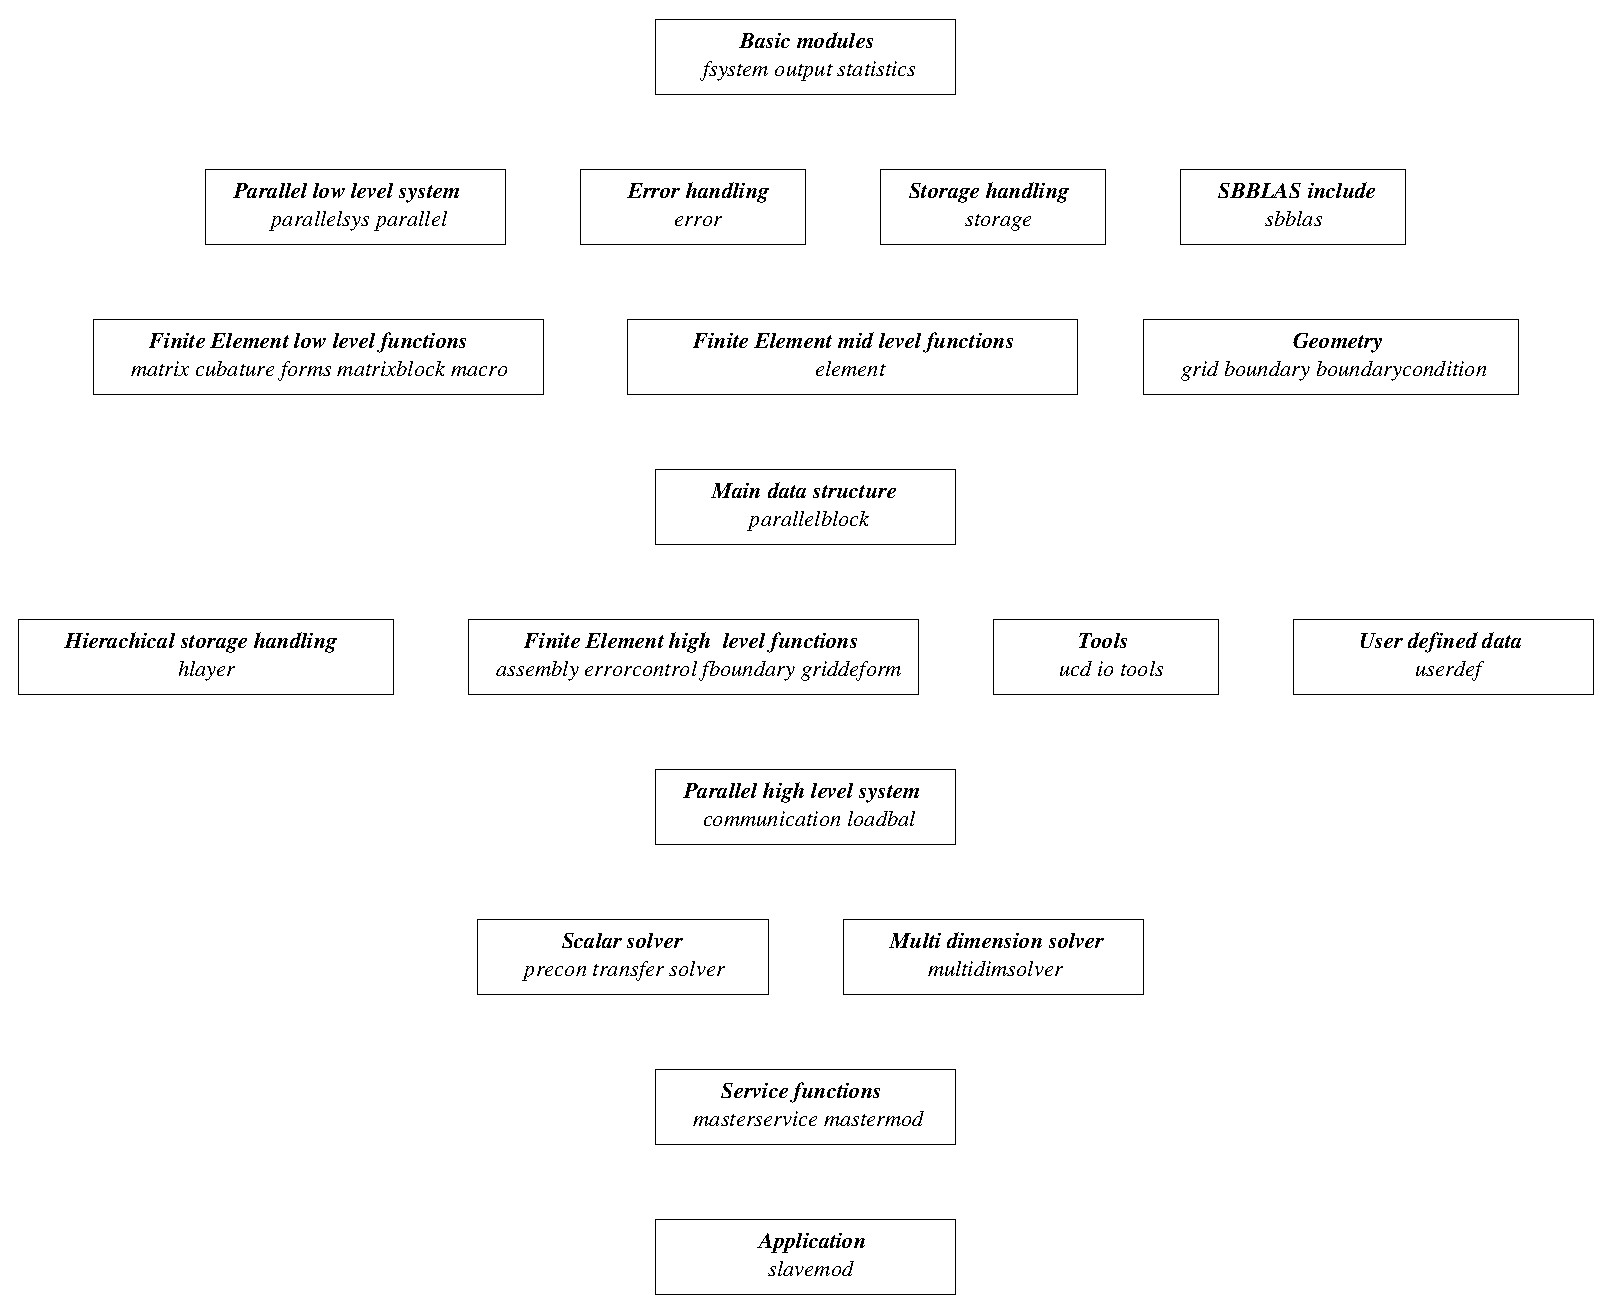
\includegraphics[scale=0.675]{../psfiles/modoverview.eps}
\end{center}
\caption{FEAST module overview}
\label{modoverview}
\end{figure}

This chapter gives a short overview of the structure of the
FEAST library and the purposes of the single modules. Figure \ref{modoverview}
shows the structure.



\include{modules_overview_dynamic}

\chapter{Module reference for application programmers}

\newpage


\include{modules_description_dynamic}


% ---- Bibliography ----
%

\bibliography{fbmathlit}

\end{document}
